\documentclass{book}
\pagestyle{plain}
\usepackage[utf8]{inputenc}
\usepackage[spanish]{babel}
\usepackage{hyperref}
\usepackage{graphicx}
\usepackage{amsmath, amssymb}
\usepackage{amsthm}          
\usepackage{textcomp}
\newtheorem*{solution}{Solución}
\usepackage{enumitem}
\usepackage{csquotes}
\usepackage{array}

\usepackage{tikz}

\begin{document}

\title{Física Acústica para Fonoaudiología}
\author{Ing. Maximiliano Adriel Ortiz}
\date{\the\year}

\maketitle

\tableofcontents

% !TeX root = ../main.tex
\chapter{Introducción}
\section{Fundamentación}

La física acústica es fundamental en la formación de un fonoaudiólogo, ya que permite comprender los principios físicos del sonido, su propagación y las características de las ondas sonoras, aspectos esenciales para evaluar y tratar trastornos de la comunicación. Con este conocimiento, el fonoaudiólogo puede entender cómo se generan, transmiten y perciben los sonidos, lo cual es crucial en la rehabilitación auditiva y del habla. Además, la física acústica ofrece herramientas para analizar la calidad del sonido y su impacto en el sistema auditivo, lo que permite mejorar las intervenciones terapéuticas y el uso de tecnologías como los audífonos.

\section{Objetivos generales y específicos}

\subsection{Objetivos generales}

\begin{itemize}
     \setlength\itemsep{0.3em}        
	\item Brindar al estudiante los elementos necesarios para alcanzar una perspectiva global del tema.
	\item Comprender y manejar los conceptos básicos de acústica y psicoacústica.

\end{itemize}   

\subsection{Objetivos específicos}  

\begin{itemize}
	\item Conocer los alcances de la acústica y su relación con la Fonoaudiología.
	\item Identificar las incumbencias del profesional en esta área.
	\item Interpretar la naturaleza del sonido y su carácter objetivo-subjetivo.
	\item Interpretar y operar con las magnitudes básicas empleadas para cuantificar los fenómenos sonoros.
	\item Entender los procesos físicos que tienen lugar en el oído humano.
        \item Caracterizar las distintas enfermedades auditivas y conocer los métodos de diagnostico de cada una.
        \item Comprender los fundamentos de los principales fenómenos psicoacusticos.
        \item Asimilar el concepto de ruido, conocer su modo de medición y sus efectos adversos.
        \item Aprender a interpretar gráficos de respuesta en frecuencia.

\end{itemize}

%%%%%%%%%%%%%%%%%%%%%%%%%%%%%%%%%%%%%%%%%%%%%%%%%%%%%%%%%%%%%%%%%%%%%%%%%%%%%%%%%%%%%%%%%%%%%%%%%%

% !TeX root = ../main.tex
\chapter{Unidad 1: Nociones básicas e introducción a la acústica}

\section{Objetivo pedagógico}
\noindent\textbf{Objetivo.} Introducir los conceptos fundamentales de la acústica, el Sistema Internacional de Unidades y las herramientas matemáticas básicas que utilizarás a lo largo de la asignatura. Estos conocimientos te permitirán entender cómo el sonido afecta la audición y la voz, y cómo se aplican en pruebas diagnósticas como audiometrías o en el diseño de audífonos. Se incluyen ejemplos, curiosidades clínicas y ejercicios pensados para estudiantes con escasa formación previa en matemáticas.

\noindent\textbf{Pregunta inicial.} ¿Alguna vez te preguntaste por qué un susurro suena diferente a un grito, o cómo un audífono mejora la audición? ¡Esta unidad te dará las bases para responder estas preguntas!

\section{¿Qué es la acústica?}
La \textbf{acústica} es la rama de la física que estudia las ondas mecánicas en gases, líquidos y sólidos. Estas ondas son vibraciones que viajan a través de un medio, como las ondas que se forman al tirar una piedra en un estanque. La acústica analiza cómo se \emph{genera} el sonido (por ejemplo, al hablar), cómo se \emph{propaga} (viaja por el aire), cómo \emph{interactúa} con el entorno (como un eco en una iglesia) y cómo lo \emph{percibe} el oído humano.

\subsection{Importancia en Fonoaudiología}
\begin{itemize}
    \item \textbf{Diagnóstico:} Las audiometrías, otoemisiones acústicas y potenciales evocados dependen de entender cómo viaja el sonido y cómo lo recibe el oído.
    \item \textbf{Rehabilitación:} El diseño de audífonos e implantes cocleares se basa en modelar la respuesta del sonido en el oído.
    \item \textbf{Análisis de la voz:} La acústica permite estudiar trastornos del habla, como la disfonía, analizando las frecuencias de la voz.
    \item \textbf{Ambientes clínicos:} Controlar el ruido de fondo en cabinas audiométricas es clave para obtener resultados precisos.
\end{itemize}

\begin{quote}
    \textbf{Dato curioso.} El término \textbf{acústica} proviene del griego \emph{akoustikos}, que significa ``relativo a la audición''. ¡Los antiguos griegos ya estudiaban cómo percibimos el sonido!
\end{quote}

\begin{figure}[h]
    \centering
    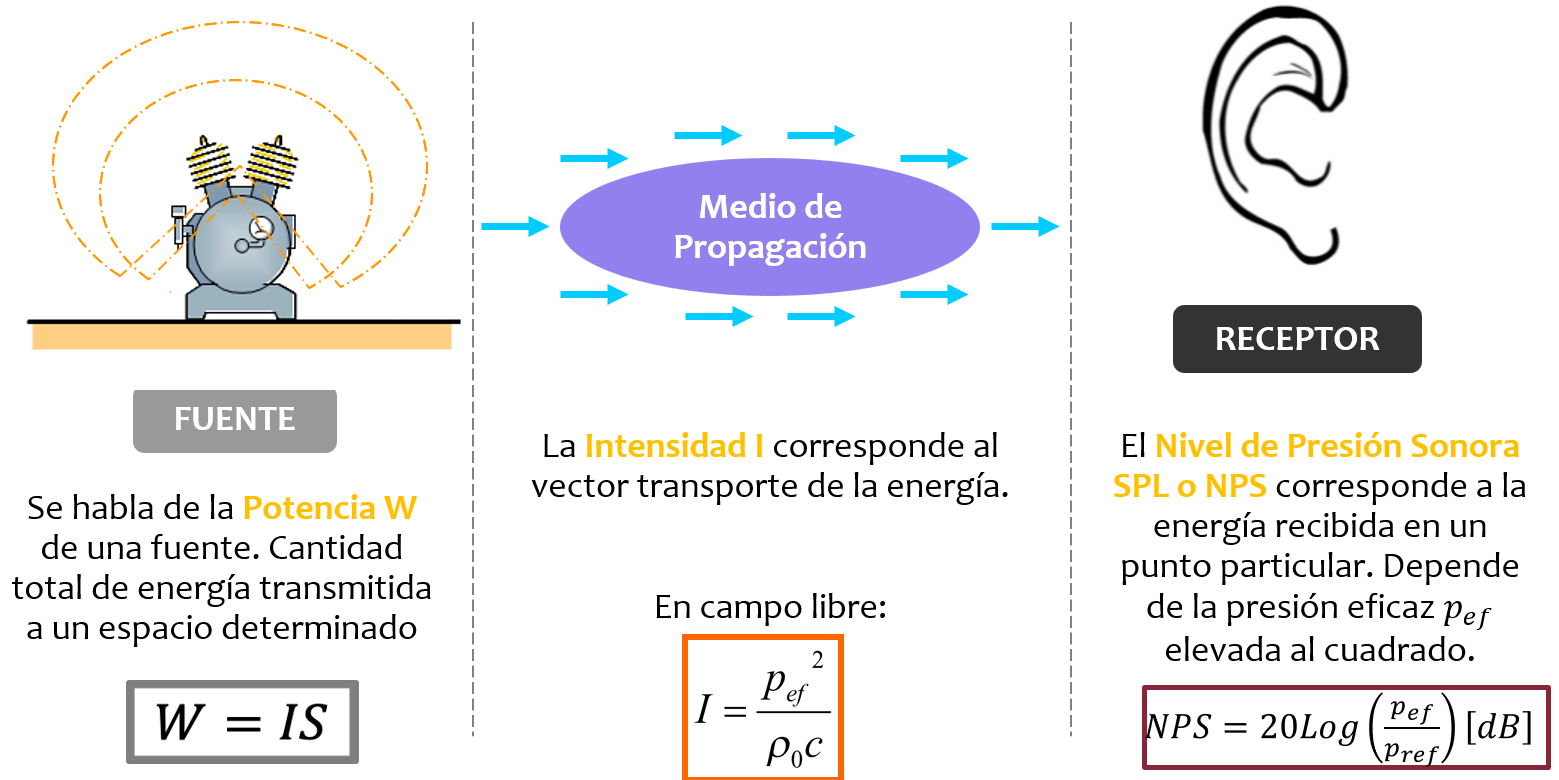
\includegraphics[width=1.0\textwidth]{figures/propagacion_sonido.png}
    \caption{ Diagrama simple de una onda sonora viajando desde una fuente hasta el oído humano a través de un medio de propagación.}
    \label{propagacion_sonido}
\end{figure}

\textbf{Recurso recomendado.} Video: \href{https://www.youtube.com/watch?v=qV4lR9EWGlY&ab_channel=CrashCourse}{``What is Sound?'' (Crash Course Physics).}  

\section{El sonido como onda mecánica}
Una onda sonora es una \emph{perturbación} que se propaga gracias a la elasticidad e inercia del medio, como el aire, el agua o el hueso. Imagina que golpeas un resorte: las compresiones viajan a lo largo de él, creando una onda. Así funciona el sonido en el aire, llevando la voz o la música hasta tu oído.

Es importante destacar que el sonido se propaga mediante ondas generadas por el movimiento oscilatorio de las partículas del medio, las cuales, tras transmitir la energía, regresan a su posición inicial. Este concepto es fundamental para comprender la transmisión del sonido en diferentes medios y será explorado en mayor detalle en capítulos posteriores.


\subsection{Tipos de ondas}
\begin{description}
    \item[\textbf{Ondas longitudinales:}] Las partículas del medio vibran en la misma dirección en que viaja la onda, creando zonas de compresión y rarefacción. Ejemplo: el sonido de tu voz viajando por el aire hasta el tímpano.
    \item[\textbf{Ondas transversales:}] Las partículas vibran perpendicularmente a la dirección de la onda. En fonoaudiología, estas ondas son relevantes en la audición ósea, cuando el cráneo vibra. Ejemplo: una cuerda de guitarra que vibra hacia arriba y abajo.
\end{description}

\begin{figure}[h]
    \centering
    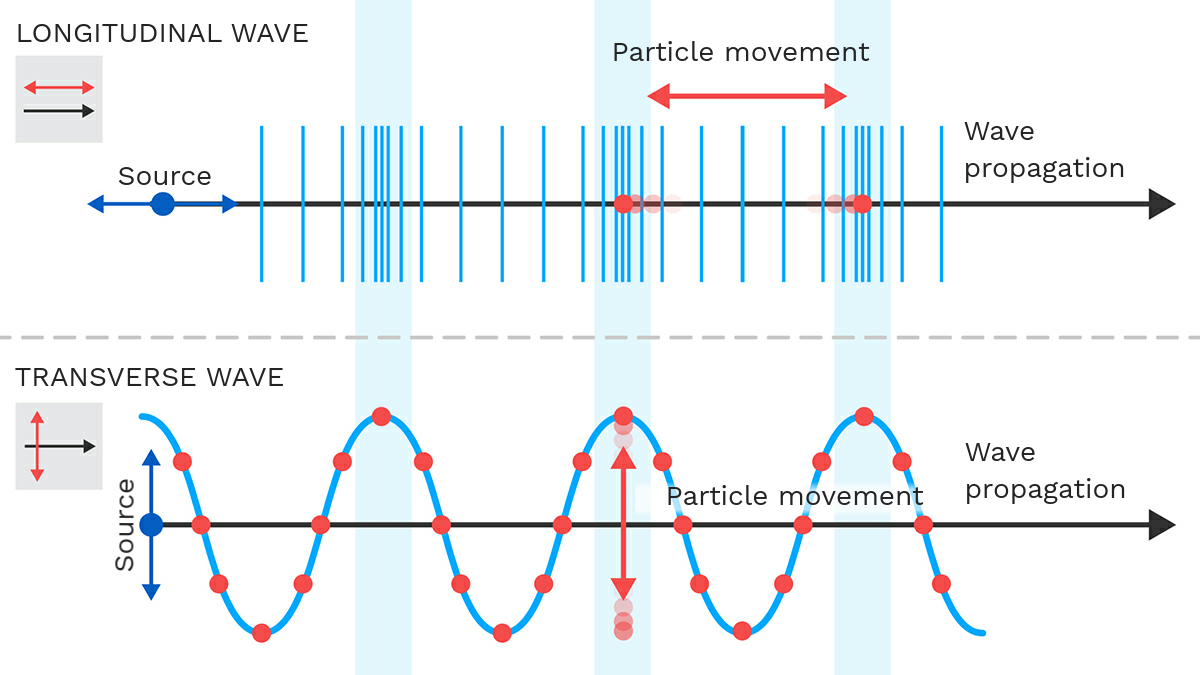
\includegraphics[width=1.0\textwidth]{figures/longitudinales_transversales.png}
    \caption{Comparativa de ondas longitudinales y transversales.}
    \label{fig:longitudinales-transversales}
\end{figure}

\textbf{Actividad práctica.} Usa un diapasón (o un video de un diapasón en YouTube) y un recipiente con agua. Golpea el diapasón para que vibre y acércalo al agua sin tocarla; escucha el sonido en el aire. Luego, sumerge parcialmente el diapasón en el agua mientras vibra y observa cómo el sonido cambia (puede sonar más apagado o diferente). Finalmente, golpea el diapasón y colócalo en una superficie sólida (como una mesa) para notar cómo las vibraciones se transmiten al medio sólido. Esta actividad muestra que el sonido necesita un medio (aire, agua o sólido) para propagarse, y que las características del medio afectan la transmisión.


\section{Sistema Internacional de Unidades (SI)}

\subsection{Magnitudes fundamentales}
En acústica, usamos unidades estándar para medir el sonido y sus efectos. Las más importantes son:

\begin{table}[h]
    \centering
    \begin{tabular}{|l|c|c|l|}
        \hline
        \textbf{Magnitud} & \textbf{Símbolo} & \textbf{Unidad (símbolo)} & \textbf{Relevancia en acústica} \\
        \hline
        Longitud & $l$ & metro (m) & Longitud de onda del sonido \\
        Masa & $m$ & kilogramo (kg) & Densidad del medio (aire, agua) \\
        Tiempo & $t$ & segundo (s) & Período de una onda sonora \\
        Temperatura & $T$ & kelvin (°C) & Afecta la velocidad del sonido \\
        \hline
    \end{tabular}
    \caption{Magnitudes fundamentales del SI relevantes en acústica.}
\end{table}

\subsection{Magnitudes derivadas frecuentes en acústica}
\begin{description}
    \item[\textbf{Velocidad:}] $v = \dfrac{\text{distancia}}{\text{tiempo}}$ (m/s). Ejemplo: la velocidad del sonido en el aire es $\approx 343$ m/s a 20°C.
    \item[\textbf{Aceleración:}] $a = \dfrac{\triangle v}{\triangle t}$ (m/s$^2$). Representa la tasa de variación de la velocidad con respecto al tiempo. En el contexto del sonido, la aceleración está relacionada con la fuerza que las ondas sonoras ejercen sobre las partículas del medio (como el aire o el tímpano), haciendo que vibren rápidamente. Por ejemplo, la vibración del tímpano responde a la aceleración de las partículas del aire inducida por la presión sonora.
    \item[\textbf{Fuerza:}] $F = m \cdot a$ (newton, N). Es el producto de la masa por la aceleración. En la audición, la fuerza se relaciona con el movimiento oscilatorio de los huesecillos del oído medio (martillo, yunque y estribo), que transmiten las vibraciones del tímpano al oído interno, amplificando la energía sonora para activar las células ciliadas de la cóclea.
    \item[\textbf{Presión:}] $p = \dfrac{F}{A}$ (pascal, Pa). Representa la fuerza por unidad de área. En el contexto del sonido, la presión sonora (medida en pascales) determina la intensidad del sonido que llega al tímpano, lo que se evalúa en audiometrías como el nivel de presión sonora (dBSPL) para determinar umbrales auditivos.
    \item[\textbf{Frecuencia:}] $f = \dfrac{1}{T}$ (hertz, Hz). Indica cuántos ciclos por segundo tiene un sonido, como un tono de 1000 Hz en una prueba auditiva.
\end{description}

\begin{figure}[h]
    \centering
    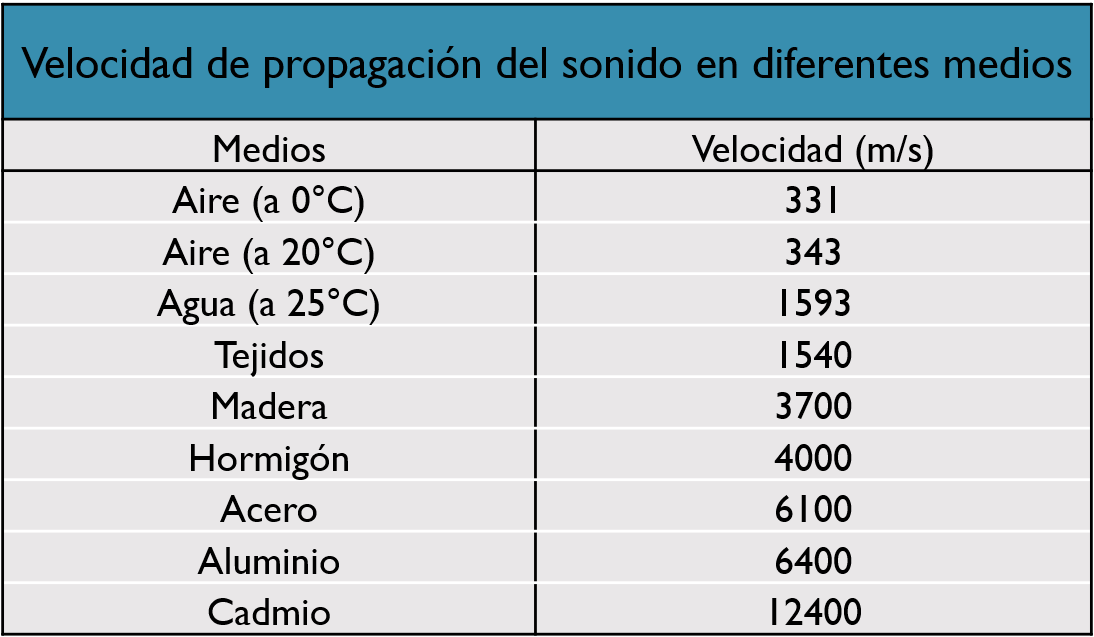
\includegraphics[width=1.0\textwidth]{figures/velocidad_propagacion_sonido.png}
    \caption{Velocidad del sonido en distintos medios de propagación}
    \label{fig:velocidad-propagacion-sonido}
\end{figure}


\subsection{Ejemplo guiado: relación distancia–velocidad–tiempo}
\begin{enumerate}
    \item \textbf{Aplauso a 100 m.} Con $c_{\text{aire}} = 343$ m/s a 20°C:
    \[
    t = \frac{100\,\text{m}}{343\,\text{m/s}} \approx 0.29\,\text{s} \Rightarrow 290\,\text{ms}.
    \]
    Esto explica el retardo entre ver y escuchar fuegos artificiales.
    
    \item \textbf{Sonido en una audiometría de campo libre.} En una cabina de 2 m, el sonido de un audiómetro tarda:
    \[
    t = \frac{2\,\text{m}}{343\,\text{m/s}} \approx 0.006\,\text{s} \Rightarrow 6\,\text{ms}.
    \]
    Este tiempo es imperceptible, pero es clave para calibrar equipos.
\end{enumerate}

\section{Herramientas matemáticas básicas}

\subsection{Funciones}
Una función es como una receta: toma un dato (como el tiempo) y lo transforma en otro (como la presión del sonido). Por ejemplo, la presión del sonido en el tímpano cambia con el tiempo, creando una gráfica que sube y baja, como las ondas del mar.

\subsection{Funciones inversas}
Las funciones inversas ``deshacen'' una operación. En acústica, usamos la inversa del logaritmo para calcular la presión del sonido a partir de un nivel en decibeles (dB).

\subsection{Trigonometría aplicada a ondas}
El sonido se representa con ondas sinusoidales, que son como curvas que suben y bajan regularmente. Por ejemplo, un tono puro (como el pitido de un audiómetro) sigue una forma matemática simple:
\[
x(t) = A \sin(2\pi f t + \varphi).
\]
\begin{itemize}
    \item \textbf{Amplitud ($A$):} Determina el volumen (en pascales, Pa).
    \item \textbf{Frecuencia ($f$):} Indica la altura del sonido (en hertz, Hz). Por ejemplo, 1000 Hz es un tono típico en audiometrías.
    \item \textbf{Periodo ($T$):} Tiempo que tarda la onda en completar un ciclo (en segundos, s). También se calcula como el inverso de la frecuenta ($T = \frac{1}{f}$)
    \item \textbf{Fase ($\varphi$):} Define el punto de partida de la onda (en radianes).
\end{itemize}

\begin{figure}[h]
    \centering
    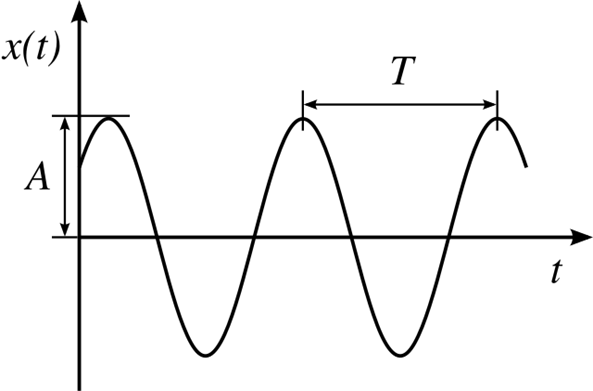
\includegraphics[width=0.8\textwidth]{figures/tono.png}
    \caption{Onda sinusoidal y sus partes.}
    \label{fig:tono-sinusoidal}
\end{figure}

\textbf{Actividad práctica.} Usa una app como Tone Generator (gratis en línea) para escuchar tonos de 250 Hz y 1000 Hz. Nota cómo el de 1000 Hz suena más agudo y prueba cambiar el volumen (amplitud).

\subsection{Logaritmos y decibel}
El oído percibe sonidos desde un susurro (20 $\mu$Pa) hasta un avión (20 Pa), un rango enorme. Los \textbf{decibeles (dB)} usan logaritmos para comprimir este rango:
\[
L_{p}\,[\text{dB}] = 20\,\log_{10}\left(\frac{p}{p_0}\right),\quad p_0 = 20\,\mu\text{Pa}.
\]
Por ejemplo, duplicar la presión del sonido aumenta 6 dB, lo que percibimos como un sonido un poco más fuerte.

\begin{table}[h]
    \centering
    \begin{tabular}{|l|c|}
        \hline
        \textbf{Sonido} & \textbf{Nivel (dB)} \\
        \hline
        Susurro & 20 \\
        Conversación normal & 60 \\
        Tráfico intenso & 80 \\
        Concierto de rock & 100 \\
        Umbral de dolor & 120 \\
        \hline
    \end{tabular}
    \caption{Niveles de decibeles de sonidos cotidianos.}
\end{table}

Video: \href{https://www.youtube.com/watch?v=XLfQpv2ZRPU&ab_channel=MED-EL}{``Understanding Sound Waves | MED-EL''}  

\textbf{Ejemplo.} Si la presión del sonido se duplica (de 20 $\mu$Pa a 40 $\mu$Pa), el nivel aumenta:
\[
\Delta L = 20 \log_{10}(2) \approx 6\,\text{dB}.
\]
Cuando ajustamos el volumen de un audífono para compensar la pérdida auditiva, lo que estamos haciendo es aumentar la presión de salida.

\section{Ejemplos prácticos}

\subsection{Conversión angular}
En acústica, los ángulos (en radianes) describen la fase de una onda. Ejemplo:
\begin{enumerate}[label=\alph*)]
    \item $90^{\circ} = \dfrac{\pi}{2}\,\text{rad}$. Esto representa un cuarto de ciclo en una onda sonora, como el desfase entre dos tonos en una prueba binaural.
    \item $640^{\circ} = 640^{\circ} - 360^{\circ} = 280^{\circ} = \dfrac{14\pi}{9}\,\text{rad}$.
\end{enumerate}

\subsection{Tiempo de viaje del sonido}
\begin{enumerate}
    \item \textbf{Delfín bajo el agua.} Un delfín a 1.5 km emite un click ($c_{\text{agua}} \approx 1500$ m/s):
    \[
    t = \frac{1500\,\text{m}}{1500\,\text{m/s}} = 1\,\text{s}.
    \]
    
    \item \textbf{Localización del sonido.} Si un sonido llega al oído derecho 0.6 ms antes que al izquierdo (distancia entre oídos $\approx 0.2$ m), el tiempo de diferencia es:
    \[
    t = \frac{0.2\,\text{m}}{343\,\text{m/s}} \approx 0.0006\,\text{s} = 0.6\,\text{ms}.
    \]
    Esto ayuda al cerebro a localizar la fuente por la diferencia interaural de tiempo, concepto que veremos en futuras unidades.
\end{enumerate}

\subsection{Nivel de presión sonora}
Para calcular el nivel de presión sonora de un tono de audiometría con presión de 0.02 Pa (20 mPa), debemos usar la siguiente formula:
\[
L_p = 20 \log_{10}\left(\frac{0.02}{20 \times 10^{-6}}\right) = 20 \log_{10}(1000) = 60\,\text{dB}.
\]
Esto corresponde a una conversación normal.

\section{Ejercicios de autoevaluación}
\begin{enumerate}
    \item Indica las unidades SI de densidad (kg/m$^3$), presión (Pa) y frecuencia angular (rad/s).
    \item Mira una gráfica de una onda sonora en una app como Audacity (puedes grabar tu voz). Identifica la amplitud (altura de la onda) y el período (distancia entre picos). Explica cómo se relacionan con el volumen y la altura del sonido.
    \item ¿Cuántos dB aumentan si la presión del sonido se multiplica por 10? (Solución: 20 dB)
    \item Escucha un tono de 500 Hz y otro de 1000 Hz usando una app como Tone Generator. ¿Cuál suena más agudo y por qué?
\end{enumerate}

\section{Glosario}
\begin{description}
    \item[\textbf{Amplitud:}] Máximo cambio de una onda respecto a su valor medio. Determina el volumen del sonido.
    \item[\textbf{Decibel:}] Unidad que mide la intensidad del sonido, basada en logaritmos.
    \item[\textbf{Fase:}] Punto de partida de una onda sonora, que afecta cómo se combina con otras ondas.
    \item[\textbf{Hz:}] Hertz, unidad de frecuencia; un ciclo por segundo.
    \item[\textbf{Onda sonora:}] Vibración que viaja por un medio, como el aire, y lleva el sonido.
    \item[\textbf{Pa:}] Pascal, unidad de presión. Mide la fuerza del sonido en el tímpano.
\end{description}

\section{Resumen}
\begin{itemize}
    \item \textbf{¿Qué es la acústica?} Estudia cómo se generan, propagan y perciben las ondas sonoras, clave en fonoaudiología para audiometrías, audífonos y análisis de voz.
    \item \textbf{Unidades clave:} Longitud (m), tiempo (s), presión (Pa), frecuencia (Hz).
    \item \textbf{Ondas sonoras:} Son longitudinales en el aire (compresiones y rarefacciones) y transversales en sólidos (como el cráneo).
    \item \textbf{Decibeles:} Miden la intensidad del sonido en una escala logarítmica, imitando cómo percibimos los cambios de volumen.
\end{itemize}

\bigskip
\noindent\emph{Conclusión.} Comprender la naturaleza del sonido, las unidades de medida y las herramientas matemáticas básicas es el primer paso para dominar la acústica. Estos conceptos te ayudarán a entender cómo se realizan audiometrías o cómo se analiza la voz de un paciente. En la próxima unidad, exploraremos cómo las leyes de Newton explican el movimiento del tímpano y los huesecillos del oído, conectando la física con la audición.


%%%%%%%%%%%%%%%%%%%%%%%%%%%%%%%%%%%%%%%%%%%%%%%%%%%%%%%%%%%%%%%%%%%%%%%%%%%%%%%%%%%%%%%%%%%%%%%%%%

% !TeX root = ../main.tex
\chapter{Unidad 2: Leyes de la mecánica clásica y de la termodinámica}

\section{Objetivo pedagógico}
\noindent\textbf{Objetivo.} Comprender cómo las leyes de Newton y los principios de la termodinámica explican la generación, propagación y transformación del sonido, conectándolos con aplicaciones en fonoaudiología, como el movimiento del tímpano, la audición ósea y el diseño de cabinas audiométricas. Se incluyen ejemplos clínicos, actividades prácticas y ejercicios de autoevaluación pensados para estudiantes con poca formación matemática.

\noindent\textbf{Pregunta inicial.} ¿Cómo logra el tímpano vibrar con el sonido de una voz? ¿Por qué el sonido cambia en un día cálido o húmedo? ¡Esta unidad te ayudará a entender estos fenómenos físicos y su impacto en la audición!

\section{Leyes de Newton y su aplicación en acústica}

Las \emph{tres leyes de Newton} describen cómo las fuerzas mueven las partículas de un medio (como el aire o los huesecillos del oído) cuando una onda sonora las atraviesa. Estas leyes son clave para entender cómo el sonido llega al oído y cómo se usa en pruebas audiométricas.

\subsection{Primera Ley (Inercia)}
Un cuerpo permanece en reposo o en movimiento uniforme a menos que una fuerza externa actúe sobre él. Imagina el tímpano como una sábana tensa: no se mueve hasta que una onda sonora la empuja.

\begin{quote}
    \textbf{Ejemplo clínico.} El tímpano está quieto hasta que una onda sonora (como el sonido de una voz) crea una diferencia de presión que lo hace vibrar. Cuando el sonido cesa, la elasticidad del tímpano lo devuelve a su posición original.
\end{quote}

\subsection{Segunda Ley (Fuerza y aceleración)}
La fuerza sobre un objeto produce una aceleración proporcional a su masa: $F = m \cdot a$. En acústica, la fuerza viene de los cambios de presión del sonido, que aceleran las partículas del aire o los huesecillos del oído.

\begin{quote}
    \textbf{Ejemplo práctico.} Cuando golpeas un diapasón, las moléculas de aire cercanas se aceleran por la presión del sonido, creando una onda que viaja hasta el oído. En el oído medio, los huesecillos (martillo, yunque y estribo) se mueven gracias a esta fuerza, amplificando el sonido. Para entender mejor este ejemplo, te invito a ver el siguiente video que muestra el \href{https://www.youtube.com/watch?v=FDMS_6ZYYbs&ab_channel=SmileandLearn-Espa%C3%B1ol}{funcionamiento del oído.}
\end{quote}

\begin{figure}[h]
    \centering
    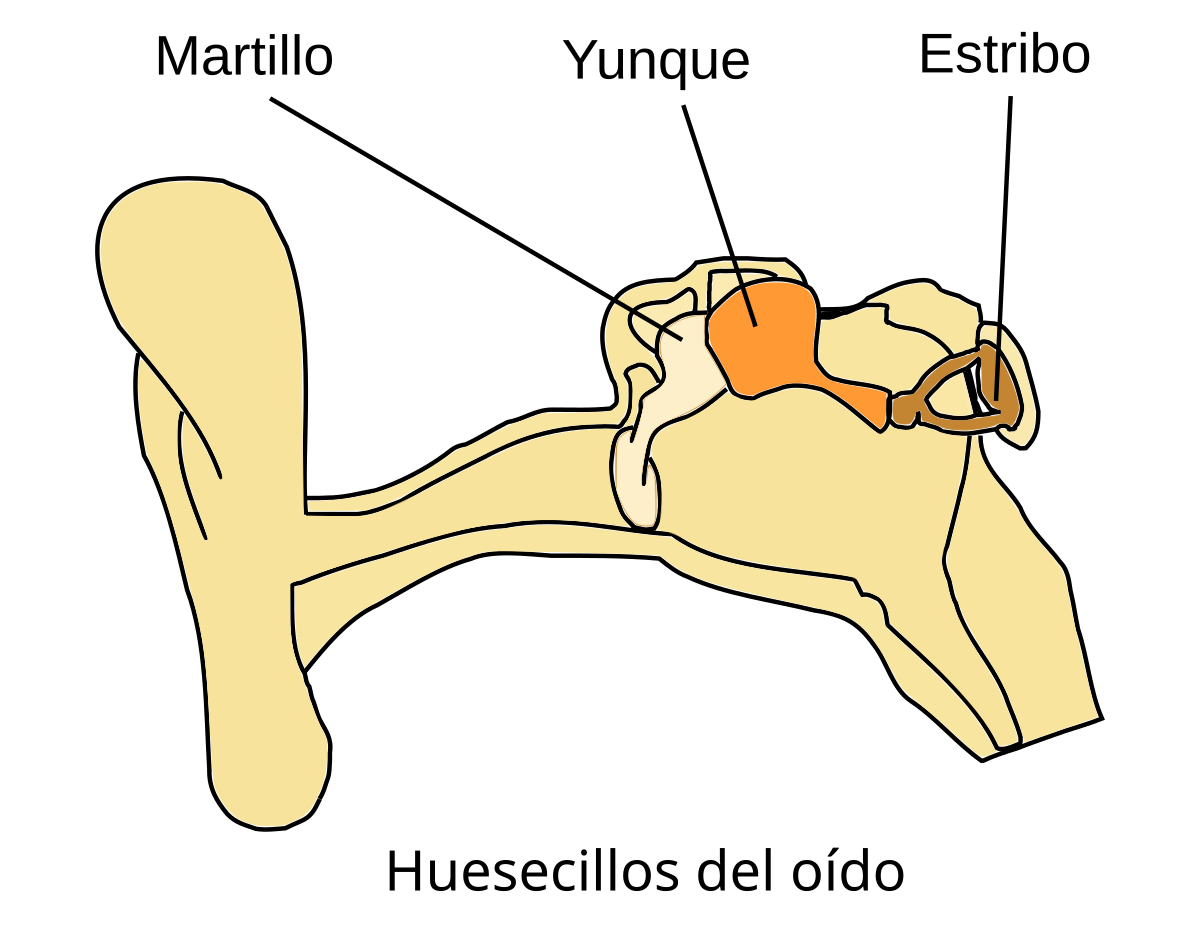
\includegraphics[width=0.6\textwidth]{figures/huesecillos.png}
    \caption{Diagrama de la cadena de huesecillos.}
    \label{huesecillos}
\end{figure}

\subsection{Tercera Ley (Acción y reacción)}
A toda acción le corresponde una reacción de igual magnitud pero con sentido opuesto. En una onda sonora, las moléculas de aire empujan a sus vecinas, que a su vez empujan de vuelta, transmitiendo el sonido en cadena.

\begin{quote}
    \textbf{Ejemplo clínico.} Cuando el estribo empuja la ventana oval en el oído interno, el líquido de la cóclea ejerce una fuerza opuesta. Esto transfiere la energía sonora al oído interno, donde se convierte en señales eléctricas.
\end{quote}

\subsection{Fricción y atenuación}
A medida que el sonido viaja, la fricción entre las moléculas de aire convierte parte de la energía en calor, reduciendo la intensidad del sonido. Este fenómeno, llamado \emph{atenuación}, es mayor en frecuencias altas (como los sonidos agudos de un silbido) y en ambientes húmedos.

\begin{quote}
    \textbf{Ejemplo práctico.} Los sonidos agudos de una voz se debilitan más rápido que los graves al viajar por el aire, lo que explica por qué escuchamos mejor los graves a la distancia.
\end{quote}

\begin{figure}[h]
    \centering
    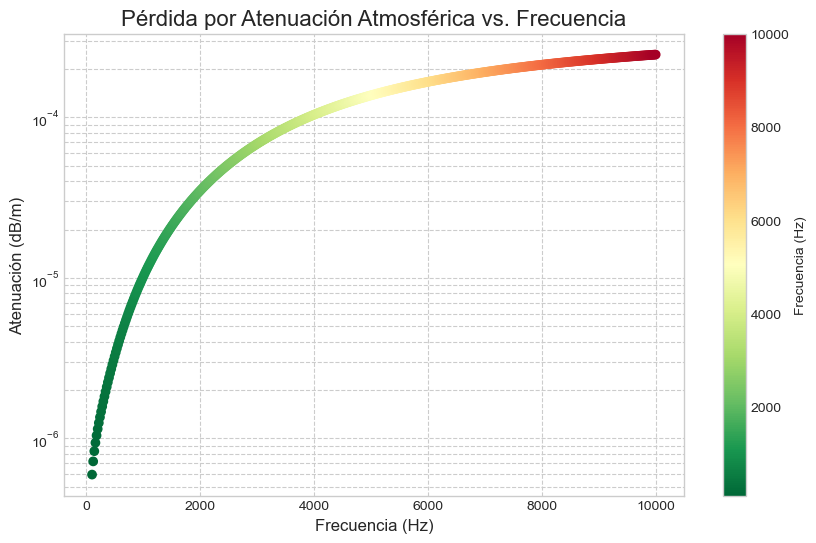
\includegraphics[width=0.8\textwidth]{figures/atenuacion_atmosferica.png}
    \caption{Fenómeno de atenuación atmosféroca.}
    \label{atenuacion_atmosferica}
\end{figure}


\section{Termodinámica del sonido}

La termodinámica estudia cómo la energía del sonido se transforma y se dispersa en el entorno. Esto es clave para entender cómo el sonido llega al oído y cómo se controla en entornos clínicos.

\subsection{Primera Ley: Conservación de la energía}
La energía no se crea ni se destruye, solo se transforma. En una onda sonora, la energía pasa de potencial (compresión del aire) a cinética (movimiento de partículas) y viceversa.

\begin{quote}
    \textbf{Ejemplo clínico.} En la cóclea, la energía mecánica del sonido (vibraciones del líquido) se transforma en energía eléctrica al activar las células ciliadas, que envían señales al cerebro.
\end{quote}

\subsection{Segunda Ley: Entropía y dispersión}
La entropía mide el desorden de un sistema. En acústica, la energía sonora tiende a dispersarse, lo que causa ecos y pérdida de claridad en espacios reverberantes. Por eso, las cabinas audiométricas están diseñadas para minimizar reflejos y mantener el sonido puro.

\begin{quote}
    \textbf{Ejemplo clínico.} En una cabina audiométrica, las paredes absorben el sonido para evitar ecos, asegurando que los tonos de la audiometría sean claros y precisos.
\end{quote}

\subsection{Temperatura y velocidad del sonido}
La velocidad del sonido depende de la temperatura del medio. En el aire, a 20°C, el sonido viaja a unos 343 m/s, pero aumenta aproximadamente 0.6 m/s por cada °C. En medios más densos, como el agua, la velocidad es mayor (1500 m/s).

\begin{table}[h]
    \centering
    \begin{tabular}{|l|c|l|}
        \hline
        \textbf{Condición} & $c$ (m/s) & \textbf{Observaciones} \\
        \hline
        $-10$~\textdegree C (aire seco) & 325 & Sonidos más apagados por alta atenuación \\
        0~\textdegree C & 331 & Referencia estándar \\
        20~\textdegree C, 50\%~RH & 343 & Condición típica en laboratorios \\
        35~\textdegree C, 90\%~RH & 352 & Mejora la inteligibilidad en exteriores \\
        \hline
    \end{tabular}
    \caption{Velocidad del sonido bajo distintas condiciones ambientales.}
\end{table}

\begin{quote}
    \textbf{Curiosidad.} Si inhalas helio, tu voz suena aguda porque el sonido viaja más rápido en helio (1000 m/s), cambiando las resonancias de tu garganta.
\end{quote}

\section{Ejemplos prácticos y autoevaluación}

\subsection{Problema resuelto: Reflejo estapedial}
El reflejo estapedial se activa a 85~dB~SPL, reduciendo el nivel a 79~dB~SPL. Calcula qué fracción de la energía acústica inicial se disipa o refleja.

\begin{quote}
    \textbf{Solución.} La diferencia es $\Delta L = 85 - 79 = 6$ dB. Esto significa que la intensidad se reduce a:
    \[
    \frac{I_2}{I_1} = 10^{-\Delta L/10} = 10^{-6/10} \approx 0.25.
    \]
    Se disipa o refleja el 75\% de la energía inicial, protegiendo el oído interno.
\end{quote}

\subsection{Ejemplo práctico: Vibración del tímpano}
El tímpano vibra con una fuerza de 0.001 N debido a un tono de 60 dB. Si su masa es aproximadamente 0.01 g (0.00001 kg), calcula la aceleración:
\[
a = \frac{F}{m} = \frac{0.001}{0.00001} = 100~\text{m/s}^2.
\]
Esto muestra cómo una pequeña fuerza produce un movimiento rápido en el tímpano.

\subsection{Ejercicios propuestos}
\begin{enumerate}
    \item \textbf{Gradiente térmico.} Dos impulsos sonoros se emiten a 500 m de distancia. En la mitad del trayecto, un frente cálido aumenta la temperatura de 20°C a 35°C. Calcula la diferencia en los tiempos de llegada. (\emph{Pista}: Usa $c = 343$ m/s a 20°C y $c = 352$ m/s a 35°C.)
    \item \textbf{Atenuación.} Un tono de 10 kHz pierde 0.2 dB por metro en aire húmedo. ¿Cuánto se atenúa tras viajar 10 m? (\emph{Solución}: 2 dB.)
    \item \textbf{Reflexión.} Explica cómo la tercera ley de Newton se aplica al movimiento de los huesecillos en el oído medio.
\end{enumerate}

\subsection{Preguntas de reflexión}
\begin{enumerate}
    \item ¿Por qué las frecuencias bajas (como un tambor) se escuchan a mayor distancia que las altas (como un silbido)?
    \item ¿Cómo ayuda una cabina audiométrica a reducir la entropía del sonido? Piensa en un consultorio con eco.
\end{enumerate}

\section{Glosario rápido}
\begin{description}
    \item[\textbf{Atenuación:}] Pérdida de intensidad del sonido debido a la fricción o dispersión en el medio.
    \item[\textbf{Entropía:}] Medida del desorden; en acústica, se relaciona con la dispersión de la energía sonora.
    \item[\textbf{Fuerza:}] Causa del movimiento, como la presión sonora que mueve el tímpano (medida en newtons, N).
    \item[\textbf{Inercia:}] Propiedad de un cuerpo para mantener su estado de reposo o movimiento.
\end{description}

\section{Resumen}
\begin{itemize}
    \item \textbf{Leyes de Newton:} Explican cómo las fuerzas del sonido mueven el tímpano y los huesecillos, esenciales para la audición.
    \item \textbf{Termodinámica:} La energía sonora se transforma (mecánica a eléctrica) y se dispersa (entropía), afectando la claridad del sonido.
    \item \textbf{Temperatura:} Afecta la velocidad del sonido (343 m/s a 20°C en aire), influyendo en la percepción y las pruebas audiométricas.
    \item \textbf{Atenuación:} Las frecuencias altas se debilitan más rápido, afectando la inteligibilidad a distancia.
\end{itemize}




\textbf{Recurso externo recomendado.} Video: \href{https://www.youtube.com/watch?v=3Br66N7QHpM&ab_channel=It%27sAumSumTime}{Why does sound travel faster in summer than in winter?.}

\bigskip
\noindent\emph{Conclusión.} Las leyes de Newton explican cómo el sonido mueve las estructuras del oído, desde el tímpano hasta la cóclea, mientras que la termodinámica nos ayuda a entender cómo la energía sonora se transforma y se pierde en el entorno. Estos principios son fundamentales para interpretar audiometrías, diseñar cabinas sonoamortiguadas y analizar cómo el ambiente afecta la voz y la audición. En la próxima unidad, exploraremos las ondas sonoras en detalle, conectándolas con la percepción auditiva.



%%%%%%%%%%%%%%%%%%%%%%%%%%%%%%%%%%%%%%%%%%%%%%%%%%%%%%%%%%%%%%%%%%%%%%%%%%%%%%%%%%%%%%%%%%%%%%%%%%

% !TeX root = ../main.tex
\chapter{Unidad 3: Fundamentos de la mecánica ondulatoria}

\section*{Objetivo pedagógico}
\noindent\textbf{Objetivo.} Comprender la diferencia entre movimiento oscilatorio y ondulatorio, describir el movimiento armónico simple (MAS) y relacionar sus parámetros (frecuencia, período, amplitud, fase y longitud de onda) con la propagación del sonido y su aplicación en fonoaudiología, como en las audiometrías. Se incluyen ejemplos clínicos, actividades prácticas, recursos multimedia y ejercicios de autoevaluación pensados para estudiantes con poca formación matemática.

\noindent\textbf{Pregunta inicial.} ¿Por qué un tono grave suena diferente a uno agudo? ¿Cómo se relaciona el movimiento de un parlante con el sonido que escuchamos? ¡Esta unidad te ayudará a entender cómo las ondas sonoras llevan la información auditiva!

\section{Movimiento oscilatorio versus movimiento ondulatorio}

\subsection{Movimiento oscilatorio}
El movimiento oscilatorio es el vaivén repetitivo de una partícula alrededor de un punto fijo, como un columpio que sube y baja. En acústica, las partículas de aire o el tímpano vibran de esta manera cuando una onda sonora las alcanza.

\begin{quote}
    \textbf{Ejemplo clínico.} Durante una audiometría, el tímpano oscila al recibir un tono puro, como un resorte que vibra con cada sonido.
\end{quote}

\subsection{Movimiento ondulatorio}
El movimiento ondulatorio ocurre cuando una perturbación (como el sonido) viaja a través de un medio, llevando energía sin mover la materia permanentemente. Imagina las olas en el mar: el agua sube y baja, pero la onda avanza hacia la playa.

\begin{quote}
    \textbf{Ejemplo práctico.} Cuando hablas, las vibraciones de tus cuerdas vocales crean ondas sonoras que viajan por el aire hasta el oído de quien escucha, mientras las moléculas de aire solo oscilan en su lugar.
\end{quote}


\textbf{Actividad práctica.} Toca una cuerda de guitarra o usa un diapasón (o mira un video en YouTube). Observa cómo la cuerda oscila en su lugar, pero el sonido viaja hasta tu oído. Esto muestra la diferencia entre oscilación y propagación.

\section{Movimiento armónico simple (MAS)}

El movimiento armónico simple (MAS) es un tipo de oscilación regular, como el movimiento de un péndulo. En acústica, describe cómo vibran las partículas de aire o el cono de un parlante para crear un tono puro.

Una onda sonora simple se representa como:
\[
x(t) = A \cos(2\pi f t + \varphi),
\]
donde:
\begin{itemize}
    \item \textbf{Amplitud ($A$):} La ``altura'' de la onda, que determina el nivel (en metros o pascales).
    \item \textbf{Frecuencia ($f$):} Cuántos ciclos por segundo (en hertz, Hz). Define la altura del sonido (grave o agudo).
    \item \textbf{Período ($T$):} Tiempo de un ciclo ($T = 1/f$, en segundos).
    \item \textbf{Fase ($\varphi$):} Punto de inicio de la onda (en radianes).
\end{itemize}

\begin{quote}
    \textbf{Ejemplo clínico.} En una audiometría, un tono de 1000 Hz ($T = 1/1000 = 0.001$ s) hace vibrar el tímpano con una amplitud pequeña, que el oído percibe como un sonido de intensidad moderada.
\end{quote}

\begin{figure}[h]
    \centering
    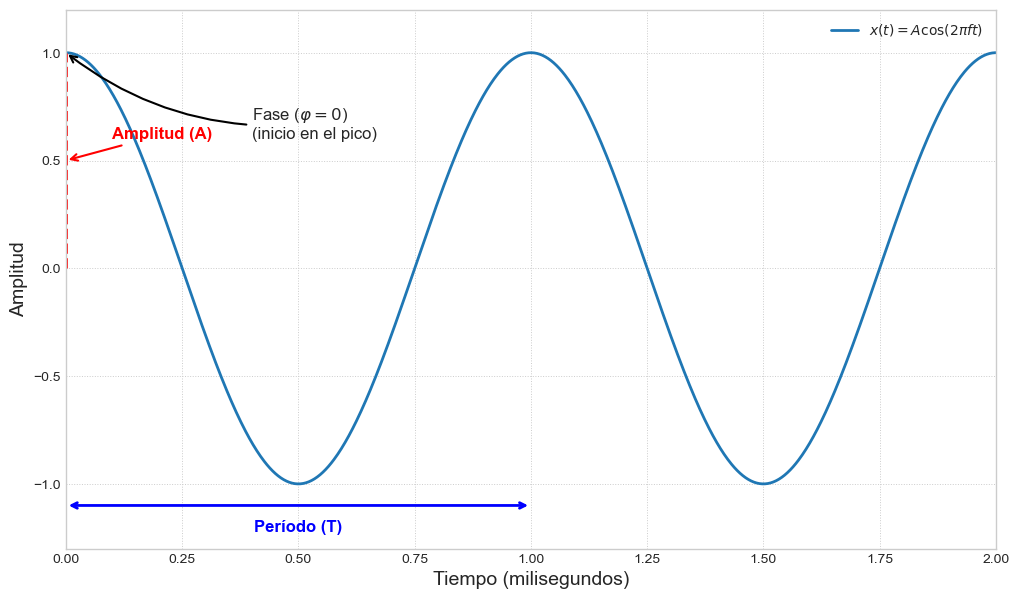
\includegraphics[width=1.0\textwidth]{figures/tono_1000.png}
    \caption{Onda sinusoidal de $f = 1000 Hz$, $A = 1$, $\phi = 0$ y $T=1, ms$.}
    \label{tono_1000}
\end{figure}


\subsection{Velocidad del movimiento}
La velocidad máxima de una partícula en MAS es:
\[
v_{\max} = 2\pi f A \quad \Biggl[\frac{m}{s}\Biggr].
\]
Por ejemplo, un parlante que vibra a 1000 Hz con una amplitud de 0.3 mm tiene una velocidad máxima de:
\[
v_{\max} = 2\pi \cdot 1000 \cdot 0.0003 \approx 1.9~\text{m/s}.
\]
Esto muestra cómo un movimiento pequeño produce un sonido audible.

\textbf{Actividad práctica.} Usa una app como Tone Generator (gratis en línea) para escuchar tonos de 250 Hz y 1000 Hz. Nota cómo el tono más agudo (1000 Hz) tiene una frecuencia mayor, lo que significa que las partículas vibran más rápido.

\section{Tono puro y su relevancia clínica}

Un \textbf{tono puro} es un sonido con una sola frecuencia, como el pitido de un audiómetro. En fonoaudiología, los tonos puros son esenciales para evaluar la audición en diferentes frecuencias (125 Hz a 8000 Hz).

\subsection{Relación longitud de onda–frecuencia}
La longitud de onda ($\lambda$) es la distancia que recorre una onda en un ciclo:
\[
\lambda = \frac{c}{f} \quad [m],
\]
donde $c$ es la velocidad del sonido (343 m/s en aire a 20°C, 1500 m/s en agua). Por ejemplo, un tono de 1000 Hz tiene:
\[
\lambda = \frac{343}{1000} \approx 0.34~\text{m} \text{ (en aire)}.
\]

\begin{table}[h]
    \centering
    \small
    \begin{tabular}{|c|c|c|c|}
        \hline
        \textbf{Frecuencia ($f$ [Hz])} & \textbf{Período ($T$ [ms])} & \textbf{$\lambda$ del aire [m]} & \textbf{$\lambda$ del agua [m]} \\
        \hline
        125 & 8.0 & 2.74 & 12.0 \\
        1000 & 1.0 & 0.343 & 1.50 \\
        4000 & 0.25 & 0.086 & 0.375 \\
        \hline
    \end{tabular}
    \caption{Período y longitud de onda de tonos puros usados en audiometrías.}
\end{table}

\begin{quote}
    \textbf{Ejemplo clínico.} En una audiometría, un tono de 4000 Hz (longitud de onda corta) prueba la audición de frecuencias agudas, comunes en el habla (como las consonantes ``s'' o ``f'').
\end{quote}

\begin{figure}[h]
    \centering
    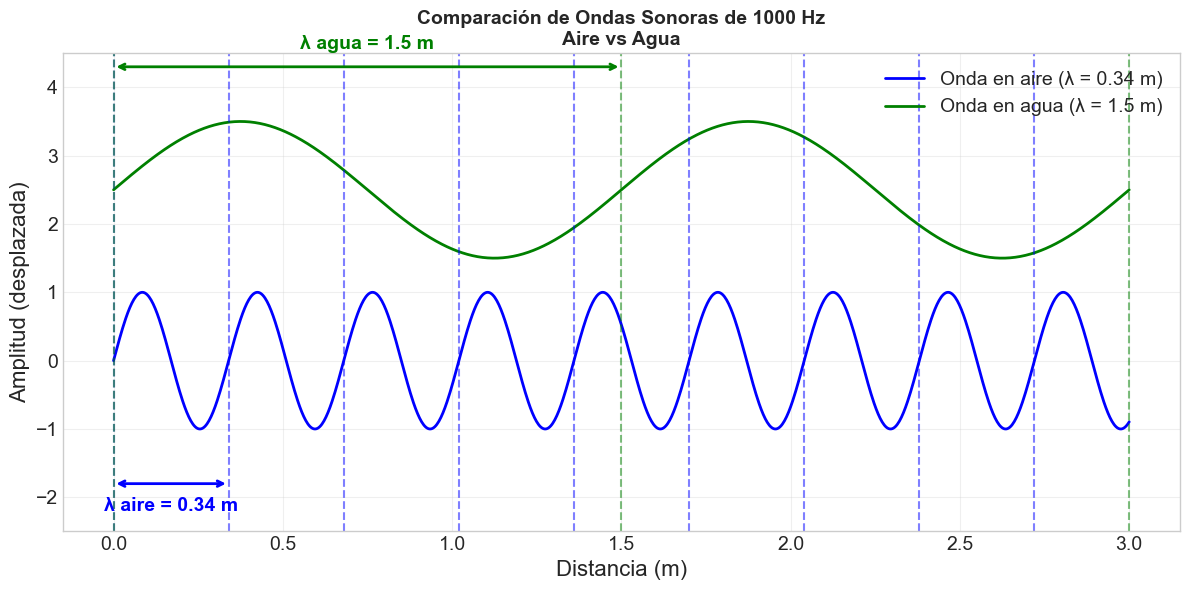
\includegraphics[width=1.0\textwidth]{figures/ondas_aire_agua.png}
    \caption{Logitud de onda de un tono de 1000 Hz en aire vs en agua.}
    \label{fig:ondas-aire-agua}
\end{figure}


\section{Fase y superposición}

La fase ($\varphi$) determina en qué punto comienza una onda. Cuando dos ondas de la misma frecuencia se combinan, su fase relativa puede sumarlas (interferencia constructiva, $\Delta\varphi = 0$) o restarlas (interferencia destructiva, $\Delta\varphi = \pi$).

\begin{quote}
    \textbf{Ejemplo clínico.} En audífonos con cancelación activa de ruido (ANC), se genera una onda con fase opuesta al ruido ambiental, reduciendo lo que escucha el usuario. Esto mejora la claridad de la voz en entornos ruidosos.
\end{quote}

\begin{figure}[h]
    \centering
    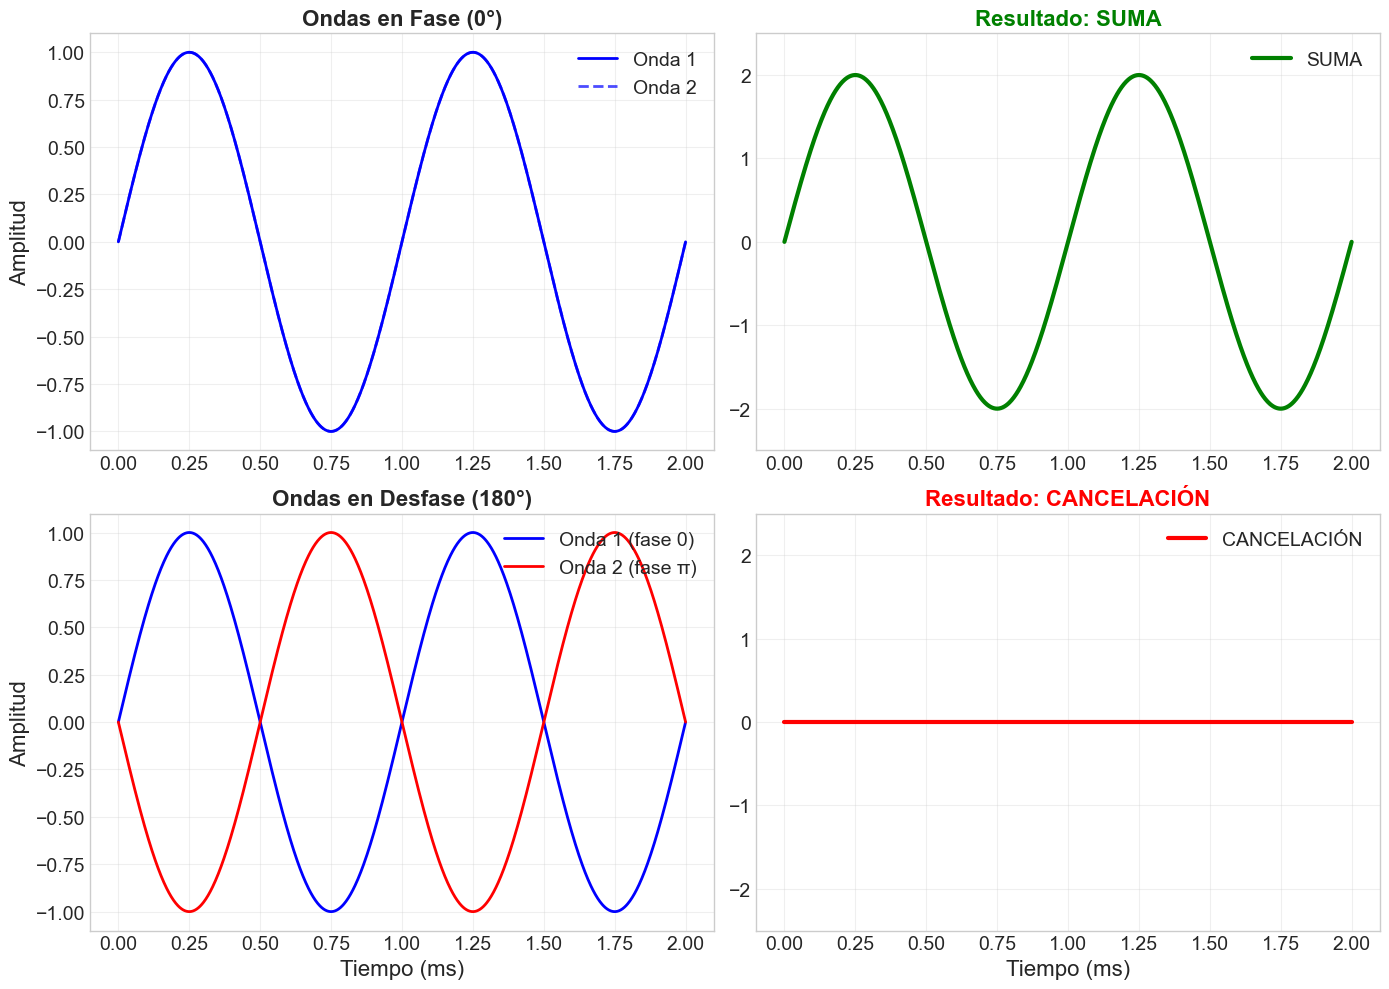
\includegraphics[width=1.0\textwidth]{figures/suma_ondas.png}
    \caption{Interferencia constructiva vs destructiva de una onda sinusoidal.}
    \label{fig:suma-ondas}
\end{figure}


\textbf{Actividad práctica.} Escucha un video de YouTube sobre cancelación de ruido (busca ``active noise cancellation'') y observa cómo los audífonos ANC reducen el ruido de fondo. Intenta identificar el principio de interferencia destructiva.

\section{Recursos recomendados}
\begin{itemize}
    \item Video: \href{https://www.youtube.com/watch?v=gZ_KnZHCn4M&ab_channel=ProfessorDaveExplains}{``Simple Harmonic Motion: Hooke's Law''}
    \item App: Tone Generator (gratis en línea). Genera tonos puros para experimentar con frecuencias.
    \item App: Audacity (gratis). Visualiza la forma de onda de tu voz o tonos puros.
    \item Libro: B. P. Kinsler \emph{et al.}, \emph{Fundamentals of Acoustics}, capítulos 4–5.
    \item Libro: L. L. Beranek, \emph{Acoustics}, sección 2.
\end{itemize}

\section{Ejemplos prácticos}

\subsection{Ejemplo 1: Cálculo de período y longitud de onda}
Para un tono de 2000 Hz en aire:
\[
T = \frac{1}{2000} = 0.5~\text{ms}, \quad \lambda = \frac{343}{2000} \approx 0.172~\text{m}.
\]
En agua:
\[
\lambda = \frac{1500}{2000} = 0.75~\text{m}.
\]
Esto muestra que las ondas son más largas en agua, afectando cómo se perciben los sonidos.

\subsection{Ejemplo 2: Velocidad de una partícula}
Un parlante vibra a 500 Hz con amplitud de 0.5 mm. La velocidad máxima es:
\[
v_{\max} = 2\pi \cdot 500 \cdot 0.0005 \approx 1.57~\text{m/s}.
\]
Esto ilustra cómo un movimiento pequeño produce un sonido audible.

\subsection{Ejemplo 3: Audiometría}
Un tono de 250 Hz ($T = 4$ ms, $\lambda = 1.37$ m en aire) se usa en una audiometría para evaluar frecuencias graves. Si el paciente no lo detecta, podría indicar pérdida auditiva en ese rango.

\section{Ejercicios de autoevaluación}
\begin{enumerate}
    \item Describe la ecuación de un MAS para un tono con amplitud de 2 mm, frecuencia de 250 Hz y fase inicial de $-\pi/4$ rad. (\emph{Solución}: $x(t) = 0.002 \cos(2\pi \cdot 250 t - \pi/4)$.)
    \item Calcula la longitud de onda en agua de un tono de 6000 Hz. (\emph{Solución}: $\lambda = 1500/6000 = 0.25$ m.)
    \item Escucha un tono de 500 Hz y otro de 2000 Hz en Tone Generator. ¿Cuál suena más agudo y por qué?
    \item Explica cómo la interferencia destructiva se usa en audífonos ANC para mejorar la audición en un entorno ruidoso.
\end{enumerate}

\section*{Glosario}
\begin{description}
    \item[\textbf{Amplitud ($A$):}] Máximo desplazamiento de una onda. Determina el volumen.
    \item[\textbf{Frecuencia ($f$):}] Número de ciclos por segundo (Hz). Define la altura del sonido.
    \item[\textbf{Período ($T$):}] Tiempo de un ciclo ($T = 1/f$). Mide la duración de una oscilación.
    \item[\textbf{Fase ($\varphi$):}] Punto de inicio de una onda, que afecta su combinación con otras.
    \item[\textbf{Longitud de onda ($\lambda$):}] Distancia entre dos puntos consecutivos en fase.
    \item[\textbf{Movimiento armónico simple (MAS):}] Oscilación regular, como la de un parlante.
    \item[\textbf{Tono puro:}] Sonido con una sola frecuencia, usado en audiometrías.
\end{description}

\section*{Resumen}
\begin{itemize}
    \item \textbf{Oscilación vs. ondulatorio:} Las partículas oscilan en su lugar, pero la onda transporta energía, como el sonido de la voz viajando al oído.
    \item \textbf{MAS:} Describe cómo vibran el tímpano o un parlante, con parámetros como amplitud (volumen) y frecuencia (altura).
    \item \textbf{Tono puro:} Esencial en audiometrías para evaluar la audición en frecuencias específicas.
    \item \textbf{Fase:} Afecta cómo se combinan las ondas, como en la cancelación de ruido.
\end{itemize}

\bigskip
\noindent\emph{Conclusión.} Comprender el movimiento oscilatorio, el movimiento armónico simple y los parámetros de las ondas (frecuencia, período, amplitud, fase, longitud de onda) es fundamental para analizar cómo se generan y propagan los sonidos. Estos conceptos te ayudarán a interpretar audiometrías, entender el diseño de audífonos y analizar fenómenos como la cancelación de ruido. En la próxima unidad, exploraremos las propiedades del sonido y su relación con la percepción auditiva.


%%%%%%%%%%%%%%%%%%%%%%%%%%%%%%%%%%%%%%%%%%%%%%%%%%%%%%%%%%%%%%%%%%%%%%%%%%%%%%%%%%%%%%%%%%%%%%%%%%

% !TeX root = ../main.tex
\chapter{Unidad 4: Generalidades sobre el sonido, sus propiedades y magnitudes}

\section*{Objetivo pedagógico}
\noindent\textbf{Objetivo.} Identificar las propiedades físicas (frecuencia, amplitud, fase) y perceptuales (altura, sonoridad) del sonido, relacionarlas con magnitudes medibles como el nivel de presión sonora (dBSPL), y aplicar las leyes de propagación (como la ley del cuadrado inverso) a problemas clínicos y de laboratorio en fonoaudiología, como audiometrías y diseño de cabinas. Se incluyen ejemplos clínicos, actividades prácticas y ejercicios de autoevaluación.

\noindent\textbf{Pregunta inicial.} ¿Por qué un grito suena más fuerte que un susurro? ¿Cómo afecta la distancia el sonido en una audiometría? ¡Esta unidad te ayudará a entender cómo medimos y percibimos el sonido!

\section{Naturaleza del sonido}
El \textbf{sonido} es una onda mecánica longitudinal que viaja a través de un medio elástico (como el aire o el agua) y es percibida por el oído como una sensación auditiva.

\begin{itemize}
    \item \textbf{Definición física:} Variaciones de presión y densidad en el medio, como las vibraciones del aire cuando hablas.
    \item \textbf{Definición psicoacústica:} La sensación que produce el sonido en el cerebro, como distinguir una voz grave de una aguda.
\end{itemize}

\subsection{Condiciones de propagación}
El sonido necesita tres elementos:
\begin{enumerate}
    \item \textbf{Fuente sonora:} Algo que vibra, como las cuerdas vocales o un parlante.
    \item \textbf{Medio elástico:} Aire, agua o hueso, que transmite las vibraciones.
    \item \textbf{Receptor:} El oído, que detecta las vibraciones y las convierte en señales nerviosas.
\end{enumerate}
Sin un medio, como en el vacío del espacio, el sonido no se propaga.

\begin{quote}
    \textbf{Ejemplo clínico.} En una audiometría, el audiómetro genera un tono puro (fuente), el aire lo lleva al tímpano (medio), y el oído lo percibe (receptor).
\end{quote}

\begin{figure}[h]
    \centering
    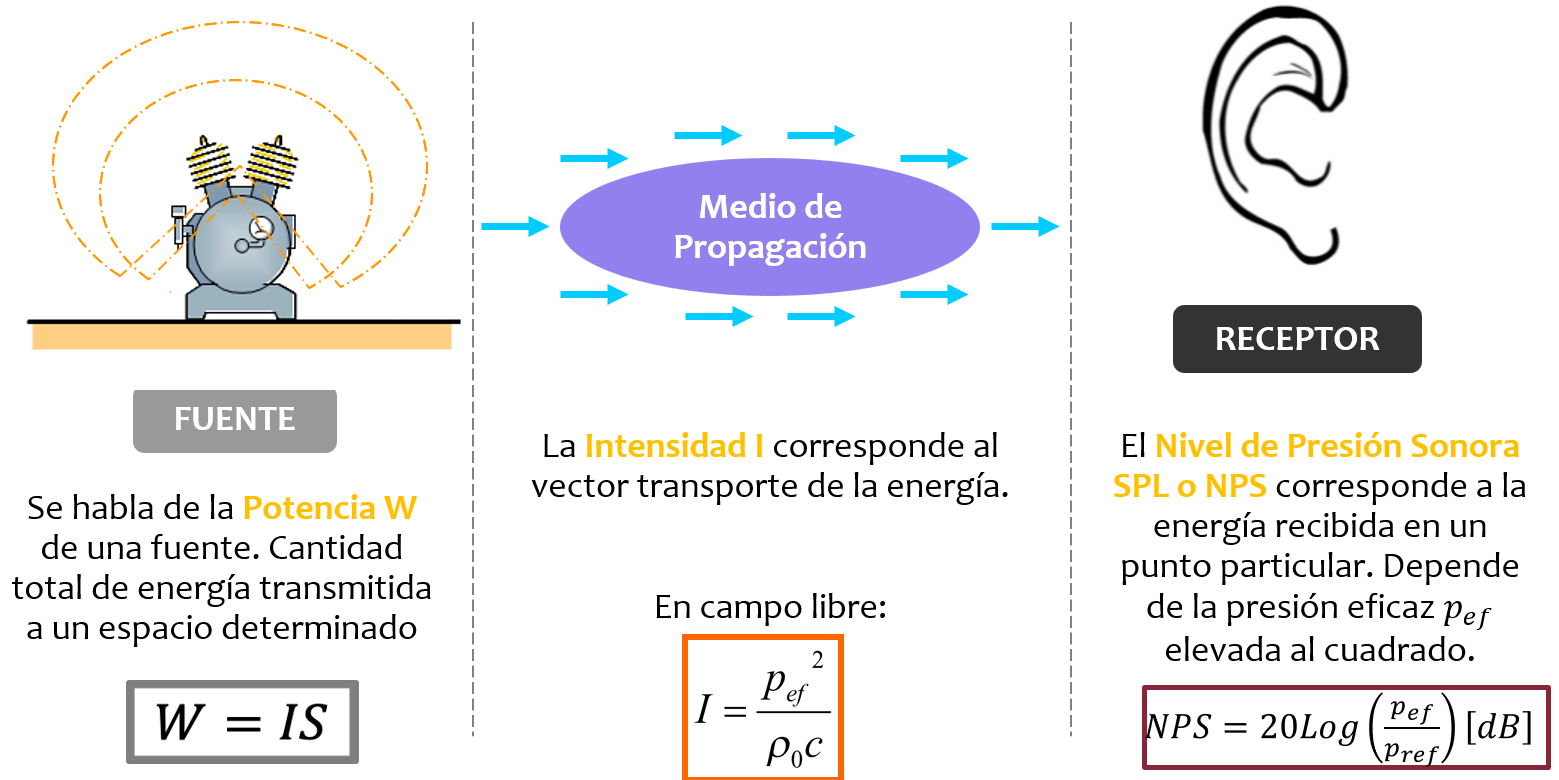
\includegraphics[width=1.0\textwidth]{figures/propagacion_sonido.png}
    \caption{Diagrama simple de una onda sonora viajando desde una fuente hasta el oído humano a través de un medio de propagación (imagen repetida de otro capítulo para afianzar el concepto).}
    \label{fig:propagacion-sonido-unidad-4}
\end{figure}

\section{Elasticidad y velocidad de propagación}
La velocidad del sonido ($c$) depende de la elasticidad ($E$, cómo el medio responde a la presión) y la densidad ($\rho$, cuánto pesan las partículas del medio):
\[
c = \sqrt{\frac{E}{\rho}}.
\]
En el aire, la velocidad aumenta con la temperatura:
\[
c \approx 331 + 0.6T \quad (\text{m/s, con } T \text{ en °C}).
\]
Por ejemplo, a 20°C, $c \approx 343$ m/s.

\begin{table}[h]
    \centering
    \begin{tabular}{|l|c|l|}
        \hline
        \textbf{Medio} & \textbf{Velocidad ($c$, m/s)} & \textbf{Observaciones} \\
        \hline
        Aire (20°C) & 343 & Condición estándar en audiometrías \\
        Agua (20°C) & 1480 & Usado en ultrasonidos médicos \\
        Hueso (aprox.) & 4000 & Relevante en audición ósea \\
        \hline
    \end{tabular}
    \caption{Velocidad del sonido en distintos medios.}
\end{table}

\begin{quote}
    \textbf{Ejemplo clínico.} En la audición ósea, el sonido viaja más rápido a través del cráneo (4000 m/s) que en el aire (343 m/s), lo que permite evaluar la cóclea directamente en pruebas audiométricas.
\end{quote}

\section{Propiedades de la onda acústica}
Las ondas sonoras tienen cuatro propiedades clave:
\begin{description}
    \item[\textbf{Frecuencia ($f$ [Hz]):}] Cuántos ciclos por segundo. Determina la \emph{altura} (grave o aguda). Por ejemplo, 250 Hz es grave (como un tambor), 4000 Hz es agudo (como una ``s'').
    \item[\textbf{Longitud de onda ($\lambda$ [m]):}] Distancia de un ciclo: $\lambda = c/f$. Una frecuencia alta tiene una longitud de onda corta.
    \item[\textbf{Amplitud ($A$ [Pa]):}] Intensidad de la variación de presión. Comúnmente esto es lo que se le dice ``volumen'' del sonido, pero en física el término preciso es ``intensidad sonora'' dado que volumen es la medida del espacio tridimensional que ocupa un cuerpo.
    \item[\textbf{Fase ($\varphi$, rad):}] Punto de inicio del ciclo. Afecta cómo se combinan las ondas.
\end{description}

\begin{quote}
    \textbf{Ejemplo clínico.} En una audiometría, se prueba la audición con tonos de diferentes frecuencias (125 Hz a 8000 Hz) para evaluar rangos graves y agudos, y con amplitudes variables para medir umbrales de audición.
\end{quote}

\section{Campo acústico}
El entorno afecta cómo percibimos el sonido:
\begin{itemize}
    \item \textbf{Campo libre:} Sin reflexiones, como en una cabina audiométrica ideal. El sonido llega directamente desde la fuente.
    \item \textbf{Campo reverberante:} Con ecos, como en una iglesia. Dificulta la claridad del habla.
    \item \textbf{Campo difuso:} Energía sonora uniforme, como en una sala ruidosa.
\end{itemize}
La \emph{distancia crítica} es el punto donde el sonido directo y los ecos tienen la misma intensidad. En cabinas audiométricas, se minimizan los ecos para garantizar mediciones precisas.

\begin{quote}
    \textbf{Ejemplo clínico.} Una cabina audiométrica usa paredes absorbentes para crear un campo libre, asegurando que el paciente escuche solo el tono puro del audiómetro.
\end{quote}

\section{Ondas esféricas y cilíndricas}
\begin{description}
    \item[\textbf{Ondas esféricas:}] Se expanden desde una fuente puntual (como un parlante) en todas direcciones. La intensidad cae 6 dB cada vez que se duplica la distancia (ley del cuadrado inverso).
    \item[\textbf{Ondas cilíndricas:}] Se propagan en un tubo o corredor (como el canal auditivo). La intensidad cae 3 dB por duplicar la distancia.
\end{description}

\begin{quote}
    \textbf{Ejemplo clínico.} En el canal auditivo, el sonido se propaga como una onda cilíndrica, lo que ayuda a amplificar frecuencias altas antes de llegar al tímpano.
\end{quote}

\begin{figure}[h]
    \centering
    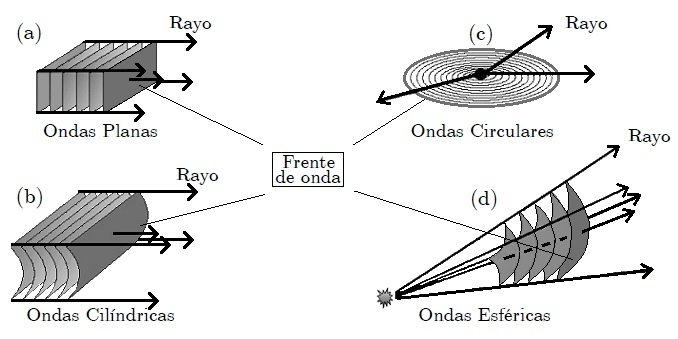
\includegraphics[width=1.0\textwidth]{figures/tipos_de_onda.jpg}
    \caption{Tipos de frente de onda.}
    \label{fig:tipos-de-onda}
\end{figure}


\section{Tono puro y señales complejas}
Un \textbf{tono puro} es un sonido con una sola frecuencia, como los tonos usados en audiometrías. Las \textbf{señales complejas} (como la voz o la música) son combinaciones de tonos puros (armónicos).

\begin{quote}
    \textbf{Ejemplo clínico.} La voz humana es una señal compleja con muchas frecuencias. En fonoaudiología, se analiza con herramientas como el espectrograma para detectar trastornos como la disfonía.
\end{quote}

\subsection{Valor RMS}
Para un tono puro, la presión RMS (raíz cuadrada media) mide la intensidad efectiva:
\[
P_{\text{RMS}} = \frac{P_0}{\sqrt{2}},
\]
donde $P_0$ es la amplitud pico. Esto se usa para calcular el nivel de presión sonora.


\begin{figure}[h]
    \centering
    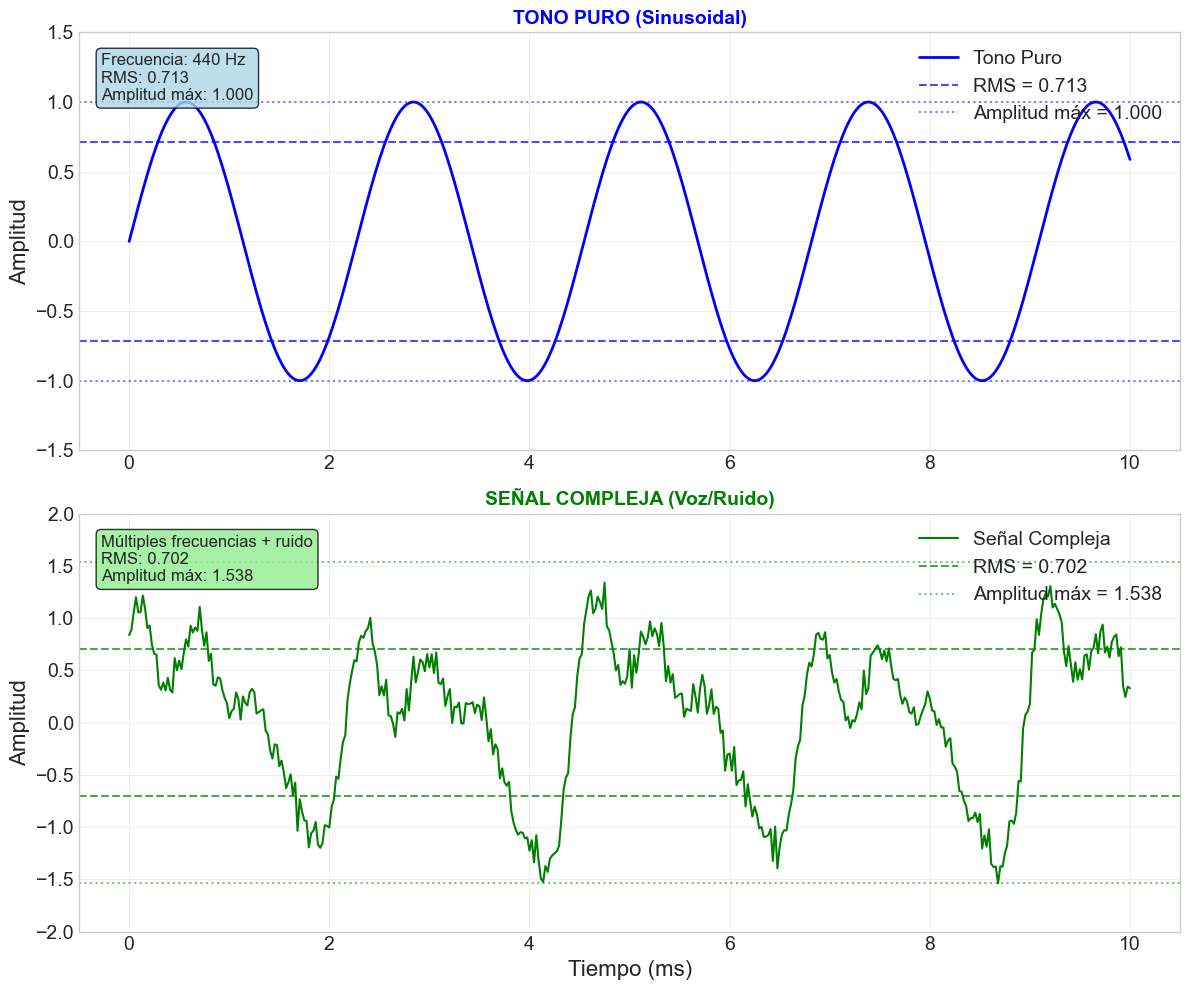
\includegraphics[width=1.0\textwidth]{figures/tono_vs_ruido.png}
    \caption{Comparación entre un tono puro y una señal compleja.}
    \label{tono_vs_ruido}
\end{figure}


\section{Presión sonora y nivel en decibeles}
El \textbf{nivel de presión sonora (SPL)} mide la intensidad del sonido en decibeles:
\[
L_p = 20 \log_{10}\left(\frac{P_{\text{RMS}}}{P_0}\right), \quad P_0 = 20~\mu\text{Pa}.
\]
La escala A (dBA) ajusta el nivel según la sensibilidad del oído humano, usada en audiometrías.

\begin{quote}
    \textbf{Ejemplo clínico.} Un tono de 60 dBA en una audiometría corresponde a una conversación normal, mientras que 20 dBA es un susurro.
\end{quote}

\section{Fuentes coherentes versus no coherentes}
\begin{description}
    \item[\textbf{Coherentes:}] Dos sonidos con la misma frecuencia y fase constante (como dos parlantes idénticos). Suman sus amplitudes, aumentando 6 dB si son iguales.
    \item[\textbf{No coherentes:}] Fases aleatorias (como dos personas hablando). Suman energías, aumentando 3 dB si los niveles son iguales.
\end{description}

\begin{figure}[h]
    \centering
    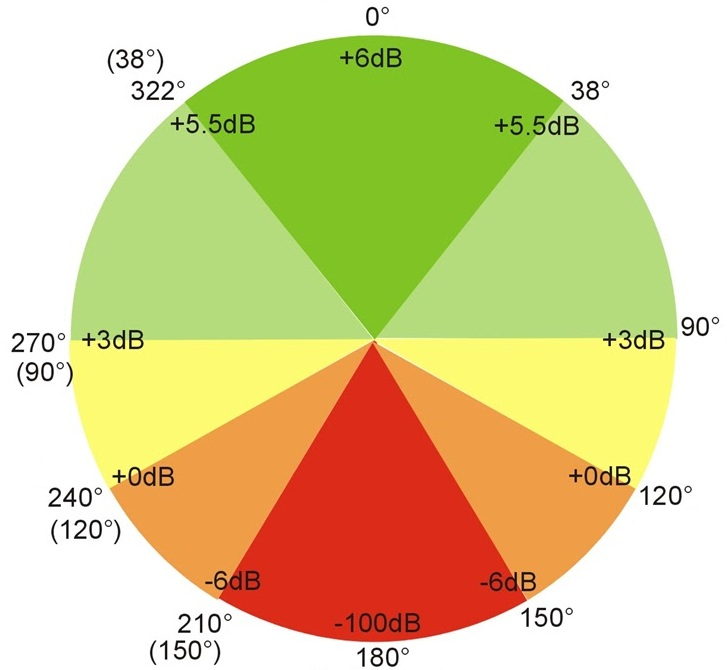
\includegraphics[width=0.6\textwidth]{figures/suma_fuentes.jpg}
    \caption{Resultado de suma de fuentes con diferente fase.}
    \label{suma_fuentes}
\end{figure}

\section{Ley del cuadrado inverso}
En un campo libre, la intensidad del sonido cae con la distancia:
\[
L_{p2} = L_{p1} - 20 \log_{10}\left(\frac{d_2}{d_1}\right).
\]
Por ejemplo, al duplicar la distancia (de 1 m a 2 m), el nivel cae 6 dB.

\begin{quote}
    \textbf{Ejemplo clínico.} Si un audiómetro produce 70 dB a 1 m en campo libre, a 2 m el nivel será 64 dB, lo que afecta la calibración en pruebas audiométricas.
\end{quote}


\section{Ejemplos prácticos}
\begin{enumerate}
    \item \textbf{Nivel a distancia.} Un altavoz omnidireccional produce 80 dB a 1 m. A 4 m:
    \[
    L_{p2} = 80 - 20 \log_{10}\left(\frac{4}{1}\right) \approx 80 - 12 = 68~\text{dB}.
    \]
    \item \textbf{Fuentes no coherentes.} Dos fuentes de 70 dB cada una suman:
    \[
    L_{\text{total}} = 10 \log_{10}(10^{70/10} + 10^{70/10}) \approx 73~\text{dB}.
    \]
    \item \textbf{Longitud de onda.} Para 500 Hz a 30°C ($c \approx 349$ m/s):
    \[
    \lambda = \frac{349}{500} \approx 0.7~\text{m}.
    \]
\end{enumerate}

\section{Ejercicios de autoevaluación}
\begin{enumerate}
    \item Explica por qué las frecuencias bajas (como un tambor) se escuchan mejor a larga distancia que las altas (como un silbido).
    \item Un audiómetro genera 70 dBSPL a 0.5 m. Calcula el nivel a 1.2 m en campo libre. (\emph{Solución}: $\approx 65.6$ dB.)
    \item En una cabina audiométrica, ¿por qué es importante minimizar las reflexiones para crear un campo libre?
\end{enumerate}

\section{Recursos recomendados}
\begin{itemize}
    \item Video: \href{https://www.youtube.com/watch?v=umTSWJ3POOk&ab_channel=AudioUniversity}{``INVERSE SQUARE LAW of Sound''}
    \item Libro: M. Raichel, \emph{Science and Applications of Acoustics}, capítulos 3–4.
    \item Libro: H. Fahy, \emph{Foundations of Engineering Acoustics}, sección 5.1.
\end{itemize}

\section*{Glosario}
\begin{description}
    \item[\textbf{Nivel de presión sonora (SPL):}] Intensidad del sonido en decibeles (dB).
    \item[\textbf{Directividad ($Q$):}] Cómo una fuente concentra el sonido en una dirección.
    \item[\textbf{Campo libre:}] Entorno sin reflexiones, ideal para audiometrías.
    \item[\textbf{Presión RMS:}] Valor efectivo de la presión sonora, usado en cálculos de dB.
    \item[\textbf{Onda longitudinal:}] Vibraciones en la dirección de propagación, como el sonido en el aire.
\end{description}

\section*{Resumen}
\begin{itemize}
    \item \textbf{Naturaleza del sonido:} Onda longitudinal que necesita fuente, medio y receptor.
    \item \textbf{Velocidad:} Depende de la elasticidad y densidad (343 m/s en aire, 4000 m/s en hueso).
    \item \textbf{Propiedades:} Frecuencia (altura), amplitud (sonoridad), fase (combinación).
    \item \textbf{Campo acústico:} Libre (sin ecos) o reverberante (con ecos), clave en cabinas.
    \item \textbf{Ley del cuadrado inverso:} La intensidad cae 6 dB al duplicar la distancia.
\end{itemize}


\bigskip
\noindent\emph{Conclusión.} Las propiedades del sonido (frecuencia, amplitud, fase) y las leyes de propagación (como la ley del cuadrado inverso) son esenciales para medir y entender la audición. Estos conceptos te ayudarán a calibrar audiómetros, diseñar entornos de prueba y analizar cómo el sonido llega al oído en diferentes condiciones. En la próxima unidad, exploraremos las herramientas para analizar y clasificar señales acústicas.


%%%%%%%%%%%%%%%%%%%%%%%%%%%%%%%%%%%%%%%%%%%%%%%%%%%%%%%%%%%%%%%%%%%%%%%%%%%%%%%%%%%%%%%%%%%%%%%%%%

% !TeX root = ../main.tex
\chapter{Unidad 5: Análisis frecuencial de señales acústicas}

\section*{Objetivo pedagógico}
\noindent\textbf{Objetivo.} Comprender cómo las herramientas de Fourier descomponen señales acústicas en sus frecuencias, explorar los rangos de frecuencia y el rango dinámico del oído humano, y aplicar filtros y curvas de ponderación (A, C, Z) en contextos clínicos de fonoaudiología, como el análisis de la voz o la calibración de cabinas audiométricas. Se incluyen ejemplos clínicos, actividades prácticas, recursos multimedia y ejercicios de autoevaluación.

\noindent\textbf{Pregunta inicial.} ¿Cómo puede un fonoaudiólogo analizar la voz de un paciente para detectar problemas? ¿Por qué algunos sonidos son más fáciles de escuchar que otros? ¡Esta unidad te ayudará a entender cómo descomponemos y medimos el sonido!

\section{Herramientas de Fourier}
Las herramientas de Fourier permiten descomponer una señal acústica (como la voz) en sus frecuencias individuales, como separar los colores de un arcoíris.

\subsection{Series de Fourier}
Una serie de Fourier es una representación matemática de una función periódica (con periodo $T$) como una suma infinita de funciones seno y coseno:
\[
x(t) = a_0 + \sum_{n=1}^{\infty} \left[ a_n \cos(2\pi n f t) + b_n \sin(2\pi n f t) \right], \quad f_0 = \frac{1}{T}
\]

La serie de Fourier descompone una función periódica en una suma de funciones senoidales y cosenoidales, cada una con una frecuencia diferente y una amplitud específica. Estas funciones senoidales y cosenoidales se denominan armónicos y la frecuencia más baja es la fundamental.

\begin{figure}[h]
    \centering
    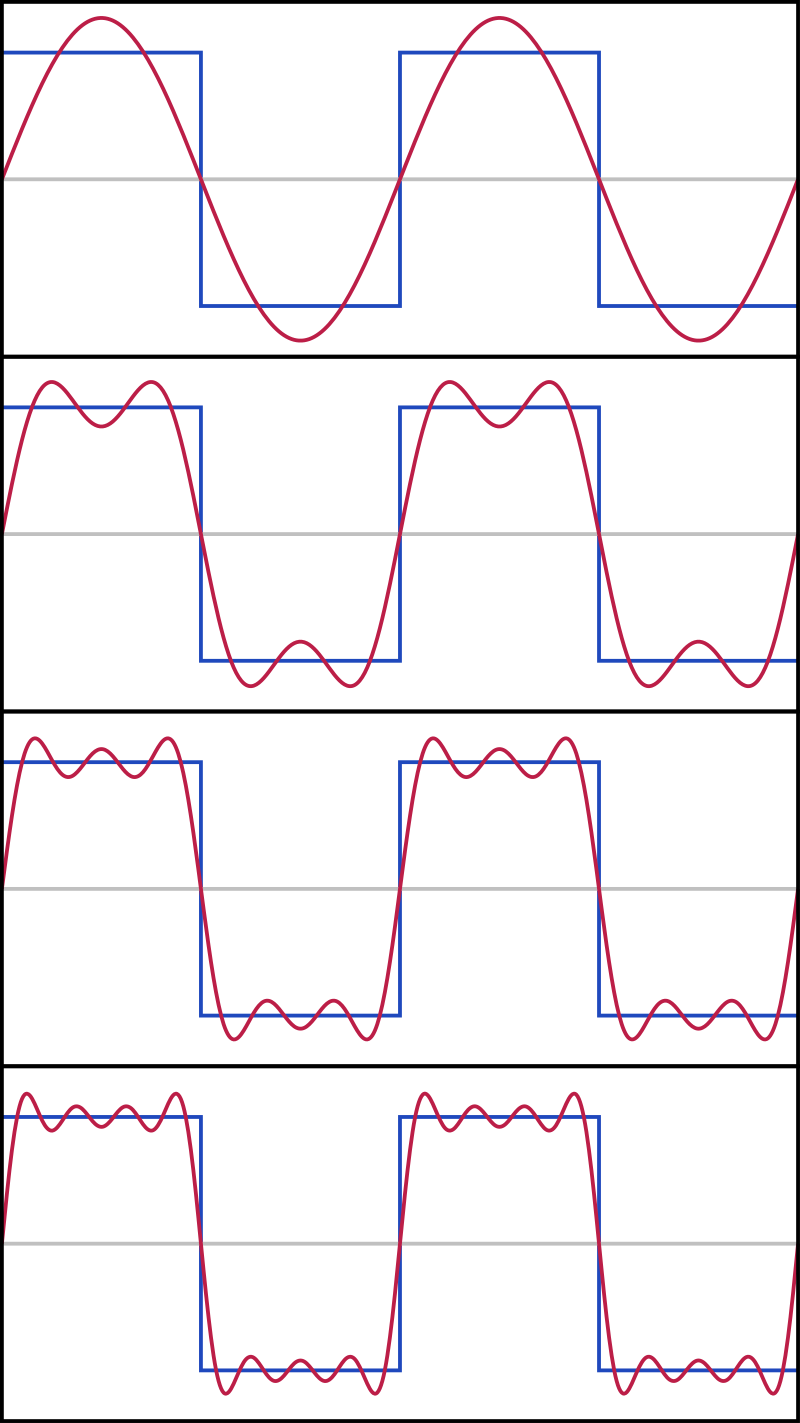
\includegraphics[width=0.4\textwidth]{figures/fourier.png}
    \caption{Aproximación a una función escalonada mediante los primeros 4 armónicos de su serie de Fourier.}
    \label{fourier}
\end{figure}

\begin{quote}
    \textbf{Ejemplo clínico.} La voz humana tiene una frecuencia fundamental ($f_0$, como 120 Hz para un hombre) y armónicos que dan su timbre único, analizados en trastornos como la disfonía.
\end{quote}

\subsection{Transformada de Fourier (FT)}
Para señales no periódicas (como una frase hablada), la transformada de Fourier muestra todas las frecuencias presentes:
\[
X(f) = \int_{-\infty}^{\infty} x(t) e^{-j 2\pi f t} \, dt.
\]
El \textbf{espectro de amplitud} ($|X(f)|$) muestra la intensidad de cada frecuencia. En la práctica, usamos la \textbf{FFT} (Transformada Rápida de Fourier) con ventanas (como Hann) para crear espectrogramas.

\begin{quote}
    \textbf{Ejemplo clínico.} Un espectrograma de la vocal /a/ muestra picos (formantes) que ayudan a diagnosticar problemas de articulación o resonancia.
\end{quote}

\begin{figure}[h]
    \centering
    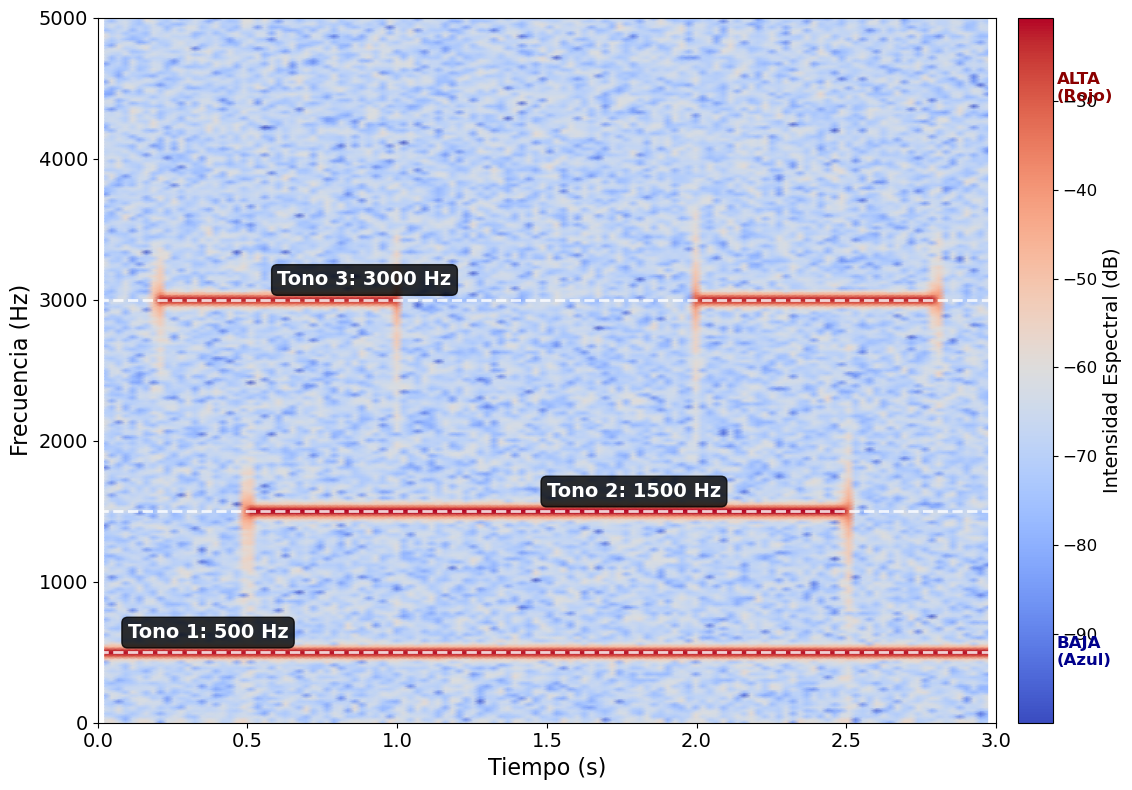
\includegraphics[width=1.0\textwidth]{figures/espectrograma.png}
    \caption{Espectrograma de una función de 3 tonos puros.}
    \label{espectrograma}
\end{figure}

\textbf{Actividad práctica.} Usa Audacity (gratis) para grabar una vocal como /a/. Ve al menú ``Análisis'' → ``Espectro'' y observa los picos de frecuencia (formantes). Compara con una vocal susurrada.

\section{Gráficos de respuesta en frecuencia}
Un gráfico de respuesta en frecuencia muestra la intensidad (en dB) frente a la frecuencia (en Hz). Los picos indican resonancias, como los formantes de la voz (F1, F2, F3), que dan el timbre.

\begin{quote}
    \textbf{Ejemplo clínico.} Un audífono se ajusta según la respuesta en frecuencia del oído del paciente, amplificando frecuencias donde hay pérdida auditiva (por ejemplo, 4000 Hz para presbiacusia).
\end{quote}

\begin{figure}[h]
    \centering
    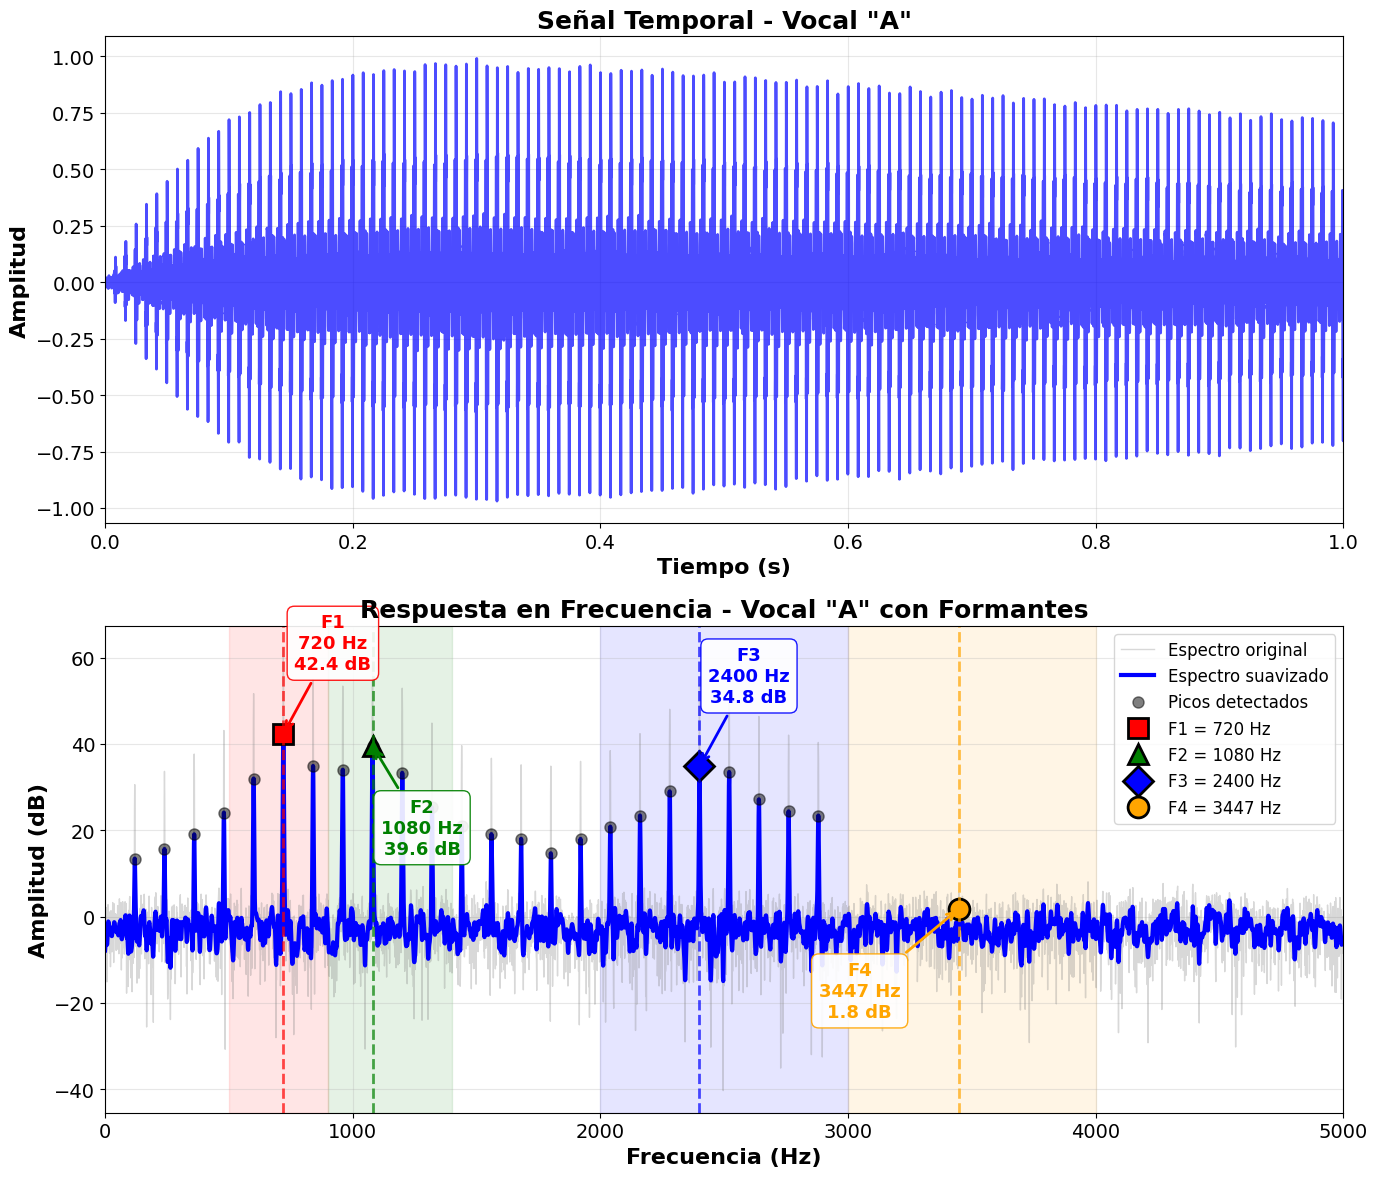
\includegraphics[width=1.0\textwidth]{figures/rta_freq_vocal.png}
    \caption{Gráfico de respuesta en frecuencia para la vocal \textit{/a/} y sus formantes.}
    \label{rta_freq_vocal}
\end{figure}


\section{Rangos de frecuencia}
El oído humano percibe sonidos en diferentes rangos:
\begin{description}
    \item[\textbf{Infrasonido:}] $<$ 20 Hz. No audible, pero puede sentirse (como vibraciones).
    \item[\textbf{Audible:}] 20 Hz a 20 kHz. Varía con la edad (los niños oyen hasta 20 kHz, en la medida que crecemos vamos perdiendo células ciliadas y nuestro rango de altas frecuencias disminuye debido a la presbiacusia).
    \item[\textbf{Ultrasonido:}] $>$ 20 kHz. Usado en pruebas médicas, como otoemisiones acústicas.
\end{description}

\subsection{Rango dinámico del oído}
El oído promedio, en el aire, detecta desde 0 dBSPL (umbral de audición) hasta 120–130 dBSPL (umbral de dolor). La voz hablada está entre 50–65 dBSPL, mientras que un susurro es~20 dBSPL.

\begin{quote}
    \textbf{Ejemplo clínico.} En una audiometría, se prueba el rango dinámico del paciente para ajustar audífonos, asegurando que los sonidos cotidianos (como la voz) sean audibles sin llegar al umbral de dolor.
\end{quote}

\section{Componentes espectrales}
Una señal acústica se compone de:
\begin{itemize}
    \item \textbf{Fundamental ($f_0$):} Frecuencia más baja en una señal compleja (por ejemplo, 120 Hz para una voz masculina).
    \item \textbf{Armónicos ($nf_0$):} Múltiplos de $f_0$, dan el timbre (por ejemplo, 240 Hz, 360 Hz).
    \item \textbf{Sobretono:} Son componentes sinusoides que se encuentran a frecuencias superiores a la fundamental. Los sobretonos que son múltiplos enteros de la fundamental se llaman \textbf{armónicos}. Los sobretonos que no son múltiplos enteros de la fundamental se denominan \textbf{inarmónicos}.
    \item \textbf{Parciales:} Son todos los componentes de frecuencia que forman la forma de onda completa, incluyendo la fundamental y los sobretonos.
    \item \textbf{Tono residual:} Percepción de $f_0$ aunque esté ausente, común en audífonos que amplifican armónicos.
\end{itemize}

\begin{figure}[h]
    \centering
    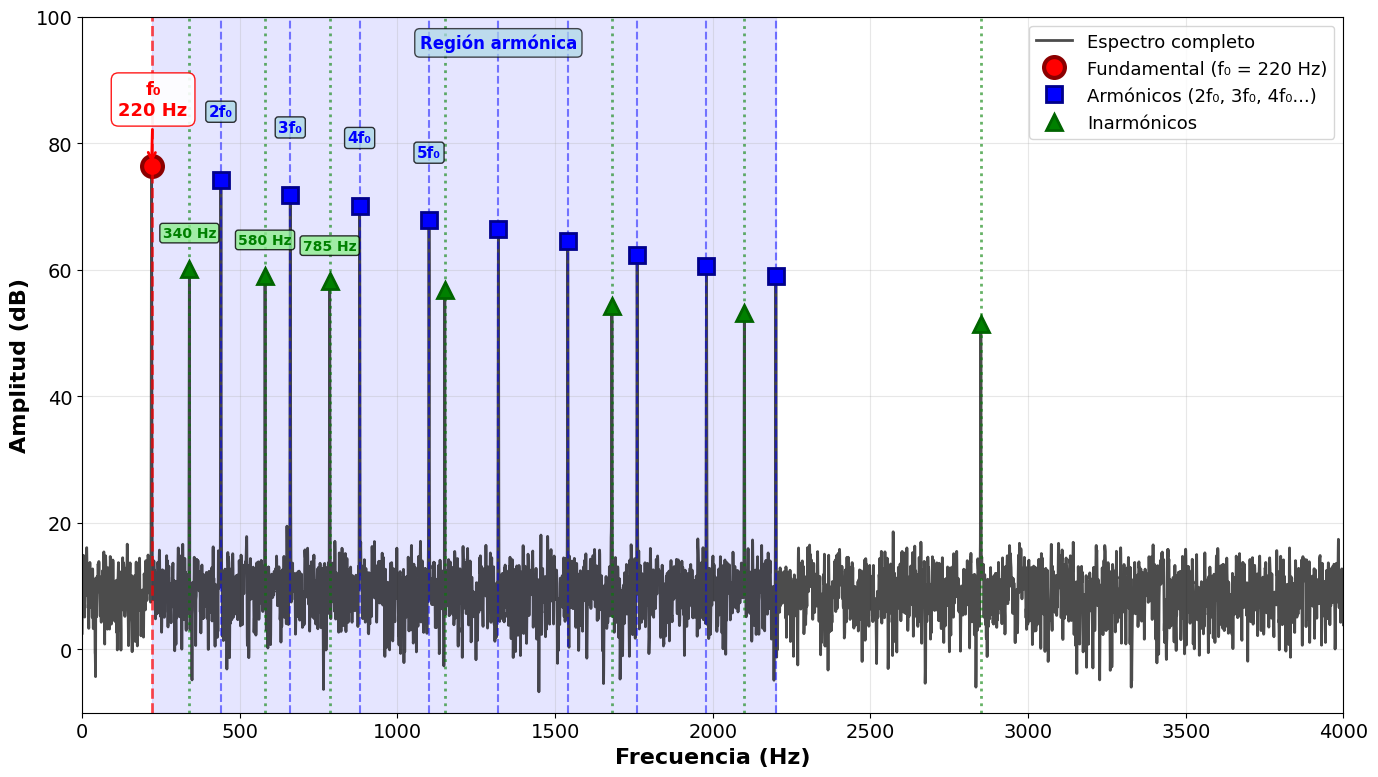
\includegraphics[width=\textwidth]{figures/armonicos.png}
    \caption{Respuesta en frecuencia de una señal marcando su fundamental, armónicos e inarmónicos.}
    \label{armonicos}
\end{figure}

\begin{quote}
    \textbf{Ejemplo clínico.} En un análisis de voz, los armónicos de una vocal ayudan a identificar si un paciente tiene disfonía (por ejemplo, armónicos débiles indican cuerdas vocales dañadas).
\end{quote}

\section{División en bandas y filtros}
Los sonidos se dividen en bandas de frecuencia para analizarlos o modificarlos.

\subsection{Bandas de octava y tercio de octava}
\begin{itemize}
    \item \textbf{Octava:} Una banda donde la frecuencia superior es el doble de la inferior ($f_{\text{sup}} = 2 f_{\text{inf}}$). Por ejemplo, 500–1000 Hz.
    \item \textbf{Tercio de octava:} Banda más estrecha, con factor $\sqrt[3]{2}$ (por ejemplo, 891–1122 Hz para una banda centrada en 1000 Hz).
\end{itemize}

\subsection{Tipos de filtros}
\begin{description}
    \item[\textbf{Pasa bajos (LPF):}] Deja pasar frecuencias bajas, atenúa las altas. Útil para eliminar ruido agudo.
    \item[\textbf{Pasa altos (HPF):}] Deja pasar frecuencias altas, atenúa las bajas. Usado en análisis de consonantes.
    \item[\textbf{Pasa banda (BP):}] Deja pasar un rango específico. Usado en audífonos para amplificar frecuencias perdidas.
    \item[\textbf{Rechaza banda (Notch):}] Elimina un rango estrecho. Útil para reducir acoples en audífonos.
\end{description}

\begin{figure}[h]
    \centering
    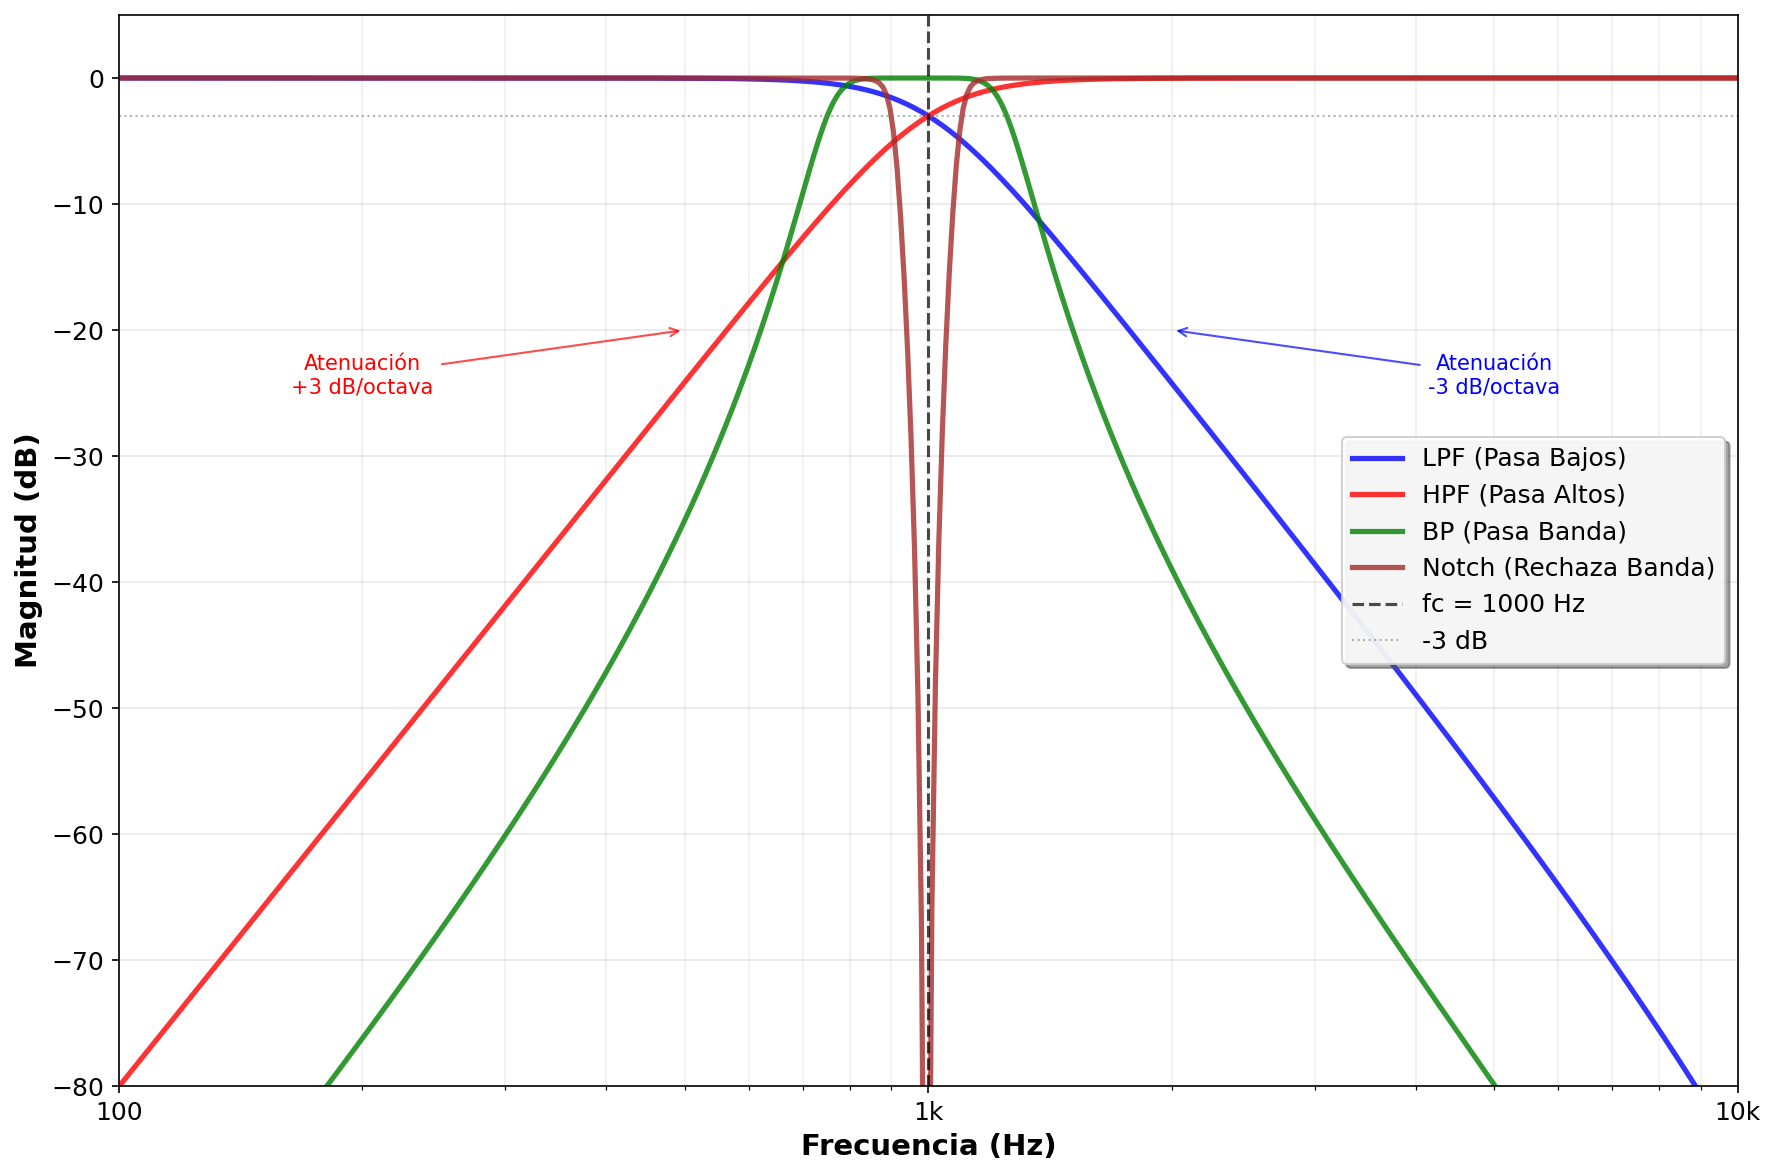
\includegraphics[width=1.0\textwidth]{figures/filtros.png}
    \caption{Diagrama comparativo de filtros LPF, HPF, BP y Notch.}
    \label{filtros}
\end{figure}

\begin{quote}
    \textbf{Ejemplo clínico.} Un audífono usa un filtro pasa banda para amplificar solo las frecuencias donde el paciente tiene pérdida auditiva (por ejemplo, 2000–4000 Hz).
\end{quote}

\textbf{Actividad práctica.} Usa Audacity para aplicar un filtro pasa bajos a una grabación de tu voz (menú ``Efectos'' → ``Filtro''). Nota cómo se eliminan los sonidos agudos (como las ``s'') y compara con un filtro pasa altos.

\section{Curvas de ponderación A, C y Z}
Las curvas de ponderación ajustan las mediciones de sonido según la sensibilidad del oído:
\begin{description}
    \item[\textbf{Curva A:}] Imita la audición a niveles moderados (50–60 dB). Atenúa bajas frecuencias. Usada en normativa de ruido laboral.
    \item[\textbf{Curva C:}] Más plana, mide niveles altos (como en conciertos).
    \item[\textbf{Curva Z:}] Sin ponderación, mide el sonido real.
\end{description}

\begin{table}[h]
    \centering
    \begin{tabular}{|c|c|c|c|}
        \hline
        \textbf{Frecuencia (Hz)} & \textbf{A (dB)} & \textbf{C (dB)} & \textbf{Z (dB)} \\
        \hline
        31.5 & -39.4 & -14.3 & 0 \\
        125 & -16.1 & -3.0 & 0 \\
        1000 & 0.0 & 0.0 & 0 \\
        8000 & +1.0 & -0.2 & 0 \\
        \hline
    \end{tabular}
    \caption{Atenuación aproximada de las curvas de ponderación (IEC 61672).}
\end{table}

\begin{figure}[h]
    \centering
    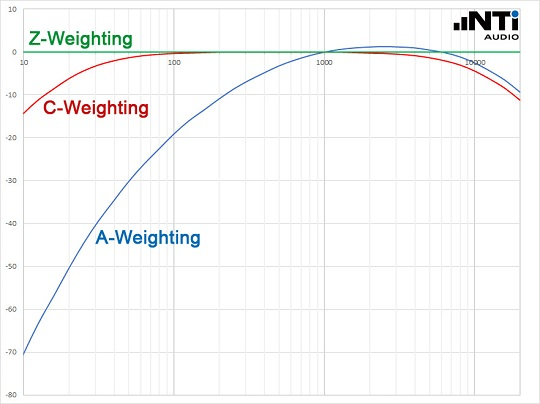
\includegraphics[width=0.8\textwidth]{figures/ponderacion.jpg}
    \caption{Curvas de ponderación A, C y Z.}
    \label{ponderacion}
\end{figure}

Los valores de atenuación para las demás frecuencias se pueden ver en este \href{https://www.nti-audio.com/es/servicio/conocimientos/ponderaciones-de-frecuencia-de-los-niveles-de-sonido}{link}. 

\begin{quote}
    \textbf{Ejemplo clínico.} En una cabina audiométrica, se usa un sonómetro con curva A para asegurar que el ruido de fondo sea < 35 dBA, garantizando pruebas precisas.
\end{quote}

\section{Medidor de nivel de presión sonora (sonómetro)}
Un sonómetro mide el nivel de presión sonora (dBSPL) y puede incluir:
\begin{itemize}
    \item \textbf{Micrófono de campo libre:} Captura el sonido sin reflexiones.
    \item \textbf{Ponderaciones A/C/Z:} Ajusta la medición según el oído humano.
    \item \textbf{Mediciones:} Instantánea (SPL), promedio ($L_{\text{eq}}$), máximo ($L_{\text{max}}$).
\end{itemize}

\begin{quote}
    \textbf{Ejemplo clínico.} Antes de una audiometría, un sonómetro verifica que el ruido en la cabina sea < 35 dBA según ISO 8253-1, asegurando resultados fiables.
\end{quote}

\section{Ejemplos prácticos}
\begin{enumerate}
    \item \textbf{Espectro de una vocal /a/.} Grabada en Audacity, muestra $f_0 = 120$ Hz (pitch), $F_1 = 730$ Hz, $F_2 = 1090$ Hz, $F_3 = 2440$, $F_4 = 3400$ Hz Hz (formantes que dan el timbre).
    \item \textbf{Filtro pasa banda.} Un filtro de 1/3 octava centrado en 1000 Hz (ancho de banda~176 Hz) aplicado a ruido rosa resalta frecuencias del habla.
    \item \textbf{Curva A.} Un tono de 63 Hz medido en 80 dB(Z) se reduce a:
    \[
    L_A = 80 - 26.2 \approx 53.8~\text{dBA}.
    \]
\end{enumerate}

\section{Ejercicios de autoevaluación}
\begin{enumerate}
    \item Usa Audacity para grabar una vocal y observa su espectro. Identifica la frecuencia fundamental ($f_0$) y al menos un formante.
    \item Calcula el nivel resultante de dos fuentes coherentes de 85 dB con diferencia de fase de 90°. (\emph{Pista:} Usa suma de fasores; solución aproximada: 88 dB.)
    \item ¿Qué atenuación aplica la curva A a un tono de 63 Hz? Usa la tabla. (\emph{Solución:} -26.2 dB.)
    \item Explica cómo un filtro pasa banda en un audífono ayuda a un paciente con pérdida auditiva en 2000–4000 Hz.
\end{enumerate}

\section{Recursos recomendados}
\begin{itemize}
    \item Video: \href{https://www.youtube.com/watch?v=r6sGWTCMz2k&ab_channel=3Blue1Brown}{``Qué es una Serie de Fourier? Del Flujo de Calor al Arte con Círculos''.}
    \item Video: \href{https://www.youtube.com/watch?v=spUNpyF58BY&ab_channel=3Blue1Brown}{``Pero, ¿qué es la transformada de Fourier? Una introducción visual.''}
    \item App: Audacity (gratis). Analiza espectros y aplica filtros.
    \item App: Decibel X (gratis). Mide niveles de presión sonora.
    \item Libro: A. Oppenheim, \emph{Signals and Systems}, capítulo 4 (introducción a Fourier).
\end{itemize}

\section*{Glosario}
\begin{description}
    \item[\textbf{FFT:}] Transformada Rápida de Fourier, para analizar frecuencias en señales.
    \item[\textbf{$L_{\text{eq}}$:}] Nivel de presión sonora promedio en un período.
    \item[\textbf{Formante:}] Pico de frecuencia en el espectro de la voz, define el timbre.
    \item[\textbf{Tercio de octava:}] Banda de frecuencia estrecha, usada en análisis acústico.
\end{description}

\section*{Resumen}
\begin{itemize}
    \item \textbf{Fourier:} Descompone señales en frecuencias (fundamental y armónicos), útil para analizar la voz.
    \item \textbf{Rangos de frecuencia:} Audible (20 Hz–20 kHz), infrasonido ($<$20 Hz), ultrasonido ($>$20 kHz).
    \item \textbf{Filtros:} Pasa bajos, pasa altos, pasa banda y Notch, usados en audífonos y análisis.
    \item \textbf{Ponderaciones A/C/Z:} Ajustan mediciones según la audición humana.
\end{itemize}

\bigskip
\noindent\emph{Conclusión.} El análisis frecuencial permite descomponer el sonido en sus componentes, identificar problemas de voz o audición, y diseñar soluciones como audífonos o cabinas audiométricas. Estas herramientas son esenciales para diagnosticar trastornos fonoaudiológicos y garantizar entornos de prueba precisos. En la próxima unidad, exploraremos cómo el cerebro procesa estas señales acústicas.



%%%%%%%%%%%%%%%%%%%%%%%%%%%%%%%%%%%%%%%%%%%%%%%%%%%%%%%%%%%%%%%%%%%%%%%%%%%%%%%%%%%%%%%%%%%%%%%%%%

% !TeX root = ../main.tex
\chapter{Unidad 6: El mecanismo de la percepción auditiva}

%------------------------------------------------
% OBJETIVO PEDAGÓGICO
%------------------------------------------------

\section*{Objetivo pedagógico}
\noindent\textbf{Objetivo.} Comprender cómo la energía acústica se transforma en señales electroquímicas que el cerebro interpreta como sonido, integrando principios físicos y neurofisiológicos para fundamentar diagnósticos y tratamientos en fonoaudiología, como audiometrías, otoemisiones acústicas (OEA), potenciales evocados auditivos (PEA), implantes cocleares y audífonos osteointegrados (BAHA). Incluye ejemplos clínicos, actividades prácticas, recursos multimedia y ejercicios de autoevaluación.

\noindent\textbf{Pregunta inicial.} ¿Cómo convierte el oído un sonido en una señal que el cerebro puede decodificar? ¿Por qué algunos pacientes perciben mejor las vibraciones a través de los huesos que por el aire? ¡Esta unidad te ayudará a develar los secretos de la audición!

%------------------------------------------------
% PANORAMA GENERAL
%------------------------------------------------

\section{Panorama general}
El sistema auditivo se organiza en cuatro grandes etapas:
\begin{enumerate}
    \item \textbf{Oído externo} – Captación y orientación del sonido.
    \item \textbf{Oído medio} – Adaptación de impedancias y protección.
    \item \textbf{Oído interno} – Análisis frecuencial y transducción mecano-eléctrica.
    \item \textbf{Vía auditiva central} – Procesamiento binaural y percepción cortical.
\end{enumerate}
Cada etapa introduce ganancias y pérdidas que permiten identificar patrones de hipoacusia conductiva, sensorioneural o retrococlear.

\begin{figure}[h]
    \centering
    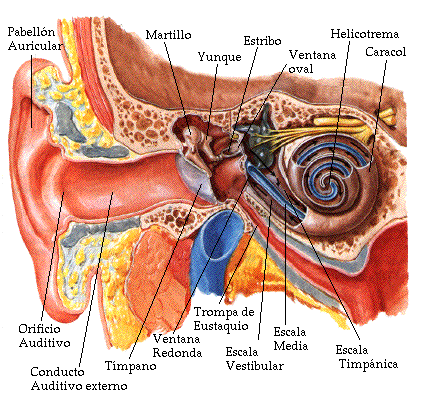
\includegraphics[width=0.8\textwidth]{figures/oido.png}
    \caption{Esquema del sistema auditivo, mostrando el oído externo, medio, interno y la vía auditiva central.}
    \label{fig:sistema_auditivo}
\end{figure}

% Nota: Reemplaza 'esquema_sistema_auditivo.jpg' con el nombre de tu archivo de imagen.

%------------------------------------------------
% OÍDO EXTERNO
%------------------------------------------------

\section{Oído externo: amplificación pasiva y orientación}
\subsection{Pabellón auricular}
El pabellón actúa como una antena direccional que filtra y amplifica frecuencias clave del habla (2–4 kHz). Su geometría genera \textit{notches} espectrales dependientes de la altura de la fuente, brindando pistas para la localización vertical del sonido.

\begin{quote}
    \textbf{Ejemplo clínico.} En casos de \emph{otia microtia} o malformaciones del pabellón, la pérdida de ganancia en altas frecuencias (2–4 kHz) afecta la discriminación de consonantes fricativas, como /s/ y /f/, esenciales para la inteligibilidad del habla.
\end{quote}

% Sugerencia: Incluir una figura del pabellón auricular mostrando los notches espectrales (e.g., \includegraphics[width=0.5\textwidth]{figures/pabellon_notches.jpg}).

\subsection{Canal auditivo externo (CAE)}
El CAE, con una longitud promedio de 27 mm, se comporta como un tubo resonador cerrado, con una frecuencia de resonancia alrededor de 3.2 kHz:
\[
f_{\mathrm{res}} = \frac{c}{4\ell} \approx \frac{343}{4 \cdot 0.027} \approx 3.2 \, \text{kHz}.
\]
Este efecto aporta entre 10 y 15 dB de ganancia en ese rango.

\begin{quote}
    \textbf{Actividad práctica.} Usa un generador de tonos a 3000 Hz (puedes emplear una app como Audacity). Observa la diferencia de sonoridad al tapar parcialmente el pabellón o al ocluir el CAE con un algodón. Opcional: graba el tono y analiza su espectro en Audacity.
\end{quote}

%------------------------------------------------
% OÍDO MEDIO
%------------------------------------------------

\section{Oído medio: adaptación de impedancias y protección}
\subsection{Transformador de impedancia acústica}
El oído medio adapta las impedancias para transferir eficientemente la energía sonora del aire al líquido del oído interno. La membrana timpánica (~60 mm$^2$) concentra la energía en la ventana oval (~3 mm$^2$), logrando una relación de 20:1. Esto, junto con la acción de palanca de la cadena osicular (1.2:1), amplifica la presión sonora, con máxima eficiencia a 1 kHz.

% Sugerencia: Incluir un esquema de la cadena osicular (e.g., \includegraphics[width=0.6\textwidth]{figures/cadena_osicular.jpg}).

\subsection{Reflejo estapedial}
Sonidos $>$ 90 dBSPL activan el músculo del estribo (latencia $\approx$ 50 ms), aumentando la impedancia para proteger la cóclea. No es efectivo ante impulsos breves (e.g., disparos). Su evaluación mediante timpanometría es clave para diagnosticar disfunciones, como en otosclerosis o lesiones del nervio facial.

\begin{quote}
    \textbf{Ejemplo clínico.} En otosclerosis, la ausencia o alteración del reflejo estapedial puede indicar fijación del estribo, observable en la timpanometría.
\end{quote}

%------------------------------------------------
% AUDICIÓN POR VÍA ÓSEA
%------------------------------------------------

\section{Audición por vía ósea}
Por encima de 50 dBSPL, las vibraciones craneales excitan el oído interno por tres rutas:
\begin{enumerate}
    \item \textbf{Inercial}: oscilación diferencial de la cadena osicular.
    \item \textbf{Compresiva}: deformación de la cápsula coclear que genera desplazamiento de perilinfa.
    \item \textbf{Osseo-timpánica}: vibración del CAE que induce movimiento timpánico.
\end{enumerate}
Este principio se aplica en audífonos osteointegrados (BAHA) y pruebas audiométricas de conducción ósea.

\begin{quote}
    \textbf{Actividad práctica.} Compara la percepción de un diapasón (vía ósea, colocado en la mastoides) con un tono por vía aérea (auriculares). Describe las diferencias en intensidad y claridad.
\end{quote}

% Sugerencia: Incluir un esquema de las rutas de conducción ósea (e.g., \includegraphics[width=0.5\textwidth]{figures/conduccion_osea.jpg}).

%------------------------------------------------
% OÍDO INTERNO
%------------------------------------------------

\section{Oído interno: análisis frecuencial y transducción}
\subsection{Arquitectura coclear y tonotopía}
La membrana basilar varía de 150 µm (base) a 450 µm (ápex). Su rigidez decreciente crea un \emph{mapa tonotópico}: 20 kHz en la base, 20 Hz en el ápex (curva de Greenwood). Cada tono activa selectivamente un segmento de ~1 mm.

% Sugerencia: Incluir un esquema de la cóclea desenrollada mostrando el mapa tonotópico (e.g., \includegraphics[width=0.7\textwidth]{figures/cochlea_tonotopia.jpg}).

\subsection{Órgano de Corti y electromotilidad de las CCE}
Las células ciliadas externas (CCE), gracias a la proteína \emph{prestina}, se contraen o alargan en microsegundos, amplificando las vibraciones de la membrana basilar hasta 40 dB y mejorando la selectividad de frecuencias.

\subsection{Evento mecano-eléctrico}
Cuando las estereocilias se mueven más de 10 nm, se abren canales (\textit{tip-links}) que permiten la entrada de iones K$^+$ desde la endolinfa (+80 mV), cambiando el voltaje de la célula (de –70 a 55 mV) y liberando glutamato hacia las neuronas aferentes.

% Sugerencia: Incluir una figura del órgano de Corti con las estereocilias y tip-links (e.g., \includegraphics[width=0.5\textwidth]{figures/organo_corti.jpg}).

%------------------------------------------------
% VÍA AUDITIVA CENTRAL Y PROCESAMIENTO BINAURAL
%------------------------------------------------

\section{Procesamiento binaural y vía auditiva central}
\subsection{Códigos binaurales}
\begin{itemize}
    \item \textbf{ITD} (\emph{Interaural Time Difference}): diferencia de tiempo/fase $<$1.5 kHz, procesada en el núcleo olivar superior medial (MSO).
    \item \textbf{ILD} (\emph{Interaural Level Difference}): sombra acústica $>$3 kHz, procesada en el núcleo olivar superior lateral (LSO).
\end{itemize}
Ambas pistas, combinadas con los \textit{notches} del pabellón, permiten localizar sonidos en 3D con una precisión angular de 1° en azimut.

\begin{quote}
    \textbf{Actividad práctica.} Con auriculares, escucha el efecto binaural \href{https://www.youtube.com/watch?v=IUDTlvagjJA&ab_channel=LovelyVirus}{“Virtual Barber Shop”}. Identifica cómo varían ITD e ILD cuando la fuente “rodea” tu cabeza. Opcional: prueba tapando un oído y describe el cambio en la percepción espacial.
\end{quote}

% Sugerencia: Incluir un diagrama de la cabeza mostrando ITD e ILD (e.g., \includegraphics[width=0.5\textwidth]{figures/binaural_cues.jpg}).

%------------------------------------------------
% APLICACIONES CLÍNICAS
%------------------------------------------------

\section{Aplicaciones clínicas principales}
\begin{itemize}
    \item \textbf{Audiometría aérea y ósea}: define el patrón de pérdida (conductiva, mixta o sensorioneural).
    \item \textbf{Otoemisiones acústicas}: TEOAE y DPOAE para cribado neonatal y monitoreo ototóxico.
    \item \textbf{Potenciales evocados auditivos} (PEA): valoración de latencias onda I–V, útil en diagnóstico retrococlear.
    \item \textbf{Impedanciometría}: timpanometría + reflejo estapedial.
    \item \textbf{Implante coclear}: estimulación eléctrica directa respetando la tonotopía, con mapeo de electrodos (20–8000 Hz).
\end{itemize}

\begin{quote}
    \textbf{Caso clínico.} Un neonato no responde al cribado con OEA. La PEA muestra latencias normales. ¿Qué pruebas adicionales recomendarías? ¿Qué tipo de hipoacusia sospecharías?
\end{quote}

% Sugerencia: Incluir un ejemplo de audiograma (e.g., \includegraphics[width=0.6\textwidth]{figures/audiograma.jpg}).

%------------------------------------------------
% EJEMPLOS PRÁCTICOS
%------------------------------------------------

\section{Ejemplos prácticos}
\begin{enumerate}
    \item \textbf{Ganancia del oído medio.} $A_t=60 \, \text{mm}^2$, $A_{vo}=3 \, \text{mm}^2$, palanca $1.2:1$. $G = 20\log_{10}\left(\frac{60}{3} \cdot 1.2\right) \approx 27.6 \, \text{dB}$.
    \item \textbf{Reflejo estapedial vs. impulso breve.} Un disparo de 120 dB, 0.1 ms, no desencadena el reflejo; riesgo de trauma acústico.
    \item \textbf{ITD máximo.} Calcula el retardo interaural máximo para una cabeza de 18 cm de diámetro:
    \[
    \Delta t_{\max} = \frac{d}{c} = \frac{0.18}{343} \approx 525 \, \mu\text{s}.
    \]
\end{enumerate}

%------------------------------------------------
% EJERCICIOS DE AUTOEVALUACIÓN
%------------------------------------------------

\section{Ejercicios de autoevaluación}
\begin{enumerate}
    \item ¿Cómo afecta la pérdida de CCE a la selectividad frecuencial? Relaciona con el ensanchamiento de las \emph{tuning curves}.
    \item Explica la diferencia entre ITD e ILD y en qué rangos de frecuencia predominan.
    \item Describe el principio de funcionamiento de un BAHA.
    \item Interpreta un audiograma con vía aérea 40 dB HL y vía ósea 10 dB HL en 500–2000 Hz.
    \item Un paciente de 60 años presenta pérdida auditiva bilateral en altas frecuencias y ausencia de reflejo estapedial. ¿Qué pruebas recomendarías y qué tipo de hipoacusia sospecharías?
\end{enumerate}

%------------------------------------------------
% RECURSOS Y BIBLIOGRAFÍA
%------------------------------------------------

\section{Recursos multimedia y bibliografía}
\begin{itemize}
    \item Video: \href{https://www.youtube.com/watch?v=jAc8A5NhJKk&ab_channel=NationalInstitutesofHealth%28NIH%29}{``El viaje del sonido al cerebro''}.
    \item Simulación: \emph{Sound Localization Demo} (MIT \slash HRTF).
    \item App: \emph{Audacity}. Visualización espectral.
    \item Simulación interactiva: \emph{Hearing Simulation} (Universidad de Minnesota, disponible en línea).
    \item Libro: Schnupp and Nelken, \emph{Auditory Neuroscience}, cap. 1–6.
    \item Libro: Pickles, \emph{Physiology of Hearing}, 4ª ed.
\end{itemize}

%------------------------------------------------
% GLOSARIO
%------------------------------------------------

\section*{Glosario}
\begin{description}
    \item[\textbf{ITD}] (\emph{Interaural Time Difference}): diferencia temporal entre oídos.
    \item[\textbf{ILD}] (\emph{Interaural Level Difference}): diferencia de nivel entre oídos.
    \item[\textbf{Prestina}] Proteína motora de las CCE responsable de la electromotilidad.
    \item[\textbf{BAHA}] (Bone-Anchored Hearing Aid): prótesis osteointegrada.
    \item[\textbf{Tuning curve}] Curva de sintonía neural.
    \item[\textbf{Tonotopía}] Organización espacial de frecuencias en la cóclea.
    \item[\textbf{Notches espectrales}] Reducciones en el espectro sonoro causadas por la geometría del pabellón.
\end{description}

%------------------------------------------------
% RESUMEN
%------------------------------------------------

\section*{Resumen}
\begin{itemize}
    \item \textbf{Oído externo}: amplifica 2–4 kHz y aporta pistas espaciales.
    \item \textbf{Oído medio}: transformador de impedancias (+27 dB) y protección.
    \item \textbf{Oído interno}: tonotopía y amplificación activa.
    \item \textbf{Vía central}: integra ITD/ILD y genera la percepción consciente.
    \item \textbf{Clínica}: audiometría, OEA, PEA, BAHA, implantes cocleares.
\end{itemize}

\bigskip
\noindent\emph{Conclusión.} La audición emerge de un delicado encadenamiento de procesos físicos, mecánicos, eléctricos y cognitivos. Conocerlos habilita intervenciones clínicas efectivas y fundamenta el diseño de tecnologías auditivas.





%%%%%%%%%%%%%%%%%%%%%%%%%%%%%%%%%%%%%%%%%%%%%%%%%%%%%%%%%%%%%%%%%%%%%%%%%%%%%%%%%%%%%%%%%%%%%%%%%%

% !TeX root = ../main.tex
\chapter{Unidad 7: Características subjetivas de la percepción auditiva (Psicoacústica)}
\section*{Objetivo pedagógico}
\noindent\textbf{Objetivo.} Explorar los atributos subjetivos del sonido (sonoridad, altura, timbre, localización, inteligibilidad), entender fenómenos como el enmascaramiento y el efecto de precedencia (Haas), y aplicar estos principios psicofísicos a la práctica fonoaudiológica, como el diseño de audífonos y la evaluación de la audición. Se incluyen ejemplos clínicos, actividades prácticas, recursos multimedia y ejercicios de autoevaluación.

\noindent\textbf{Pregunta inicial.} ¿Por qué un susurro suena más débil que un grito, aunque tengan la misma frecuencia? ¿Cómo localizamos un sonido en una sala ruidosa? ¡Esta unidad te ayudará a entender cómo percibimos el sonido!

\section{Sonoridad e igual sonoridad}

\subsection{Curvas isofónicas ISO 226 (2003)}
Las curvas isofónicas muestran cómo diferentes frecuencias y niveles de presión sonora (dBSPL) producen la misma \textbf{sonoridad} (en fones). A 1 kHz, 1 fon = 1 dBSPL. A niveles bajos ($<$40 fones), el oído es menos sensible a frecuencias graves ($<$250 Hz) y muy agudas ($>$8 kHz).

\begin{quote}
    \textbf{Ejemplo clínico.} En una audiometría, un tono de 125 Hz a 40 dBSPL se percibe más débil que uno de 1 kHz a 40 dBSPL, debido a la menor sensibilidad del oído a bajas frecuencias.
\end{quote}


\begin{figure}[h]
    \centering
    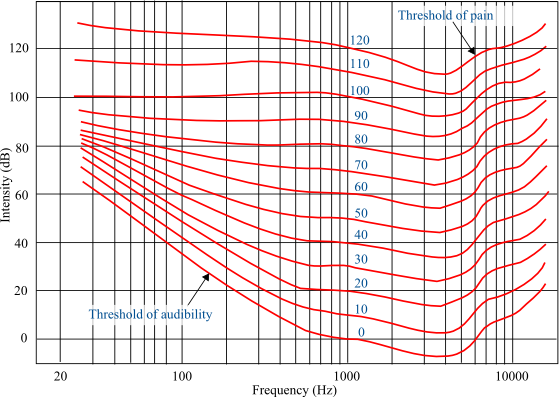
\includegraphics[width=0.9\textwidth]{figures/FletcherMunson.png}
    \caption{Curvas isofónicas de Fletcher y Munson.}
    \label{fig:isofonicas}
\end{figure}



\subsection{Ley de Stevens y conversión a sones}
La escala de \textbf{sones} mide la sonoridad de forma lineal:
\[
\text{sones} = 2^{\frac{\text{fones} - 40}{10}}.
\]
Por ejemplo, 70 fones = $2^{(70-40)/10} = 8$ sones, percibido como 8 veces más intenso que 40 fones (1 son).

\begin{quote}
    \textbf{Ejemplo clínico.} Al ajustar un audífono, aumentar de 70 dBSPL (8 sones) a 80 dBSPL (16 sones) a 1 kHz duplica la sonoridad, pero puede causar molestias si no se calibra cuidadosamente.
\end{quote}

\textbf{Actividad práctica.} Usa Tone Generator (gratis en línea) para comparar un tono de 1 kHz a 40 dB con uno de 125 Hz a 40 dB. Nota cómo el tono grave se percibe más débil, reflejando las curvas isofónicas.

\section{Umbrales y resonancia del CAE}
El \textbf{umbral absoluto} de audición es aproximadamente 0 dBSPL a 1 kHz en un campo libre (sin reflexiones). El canal auditivo externo (CAE) amplifica frecuencias de 2–4 kHz en 10–15 dB debido a su resonancia ($\approx$3.4 kHz), haciendo el oído más sensible en este rango.

\begin{quote}
    \textbf{Ejemplo clínico.} En una cabina audiométrica, el ruido de fondo debe ser $<$35 dBA para no enmascarar los umbrales de audición, especialmente en frecuencias altas donde el oído es más sensible.
\end{quote}

\section{Atributos subjetivos principales}
El sonido se percibe a través de varios atributos:
\begin{description}
    \item[\textbf{Altura (pitch):}] Depende de la frecuencia fundamental ($f_0$). Por ejemplo, 120 Hz suena grave (voz masculina), 250 Hz más agudo (voz femenina). El \textbf{pitch residual} ocurre cuando el cerebro reconstruye $f_0$ aunque esté ausente.
    \item[\textbf{Timbre:}] Determinado por los armónicos y su evolución. Diferencia un violín de una flauta, o la voz de un paciente con disfonía.
    \item[\textbf{Sonoridad:}] Relacionada con la amplitud y el ancho de banda. Un ruido amplio (como el viento) suena más fuerte que un tono puro al mismo nivel dB.
    \item[\textbf{Duración subjetiva:}] Sonidos $<$200 ms parecen más cortos; el umbral temporal es $\approx$10 ms, afectando la percepción de consonantes rápidas.
\end{description}

\begin{quote}
    \textbf{Ejemplo clínico.} En la rehabilitación de pacientes con audífonos, ajustar el timbre (amplificando armónicos) mejora la claridad del habla, mientras que la sonoridad debe equilibrarse para evitar el reclutamiento.
\end{quote}

\section{Enmascaramiento y banda crítica}

\subsection{Concepto}
El \textbf{enmascaramiento} ocurre cuando un sonido (masker) eleva el umbral de detección de otro (signal). La \textbf{banda crítica} (ERB, Equivalent Rectangular Bandwidth) es el rango de frecuencias donde la energía se suma:
\[
\text{ERB} = 24.7 (4.37 f + 1) \, \text{Hz},
\]
donde $f$ está en kHz. Por ejemplo, a 1 kHz, ERB $\approx$ 108 Hz.

\begin{quote}
    \textbf{Ejemplo clínico.} En audiometría, se usa ruido de banda estrecha para enmascarar el oído contralateral, asegurando que solo el oído evaluado detecte el tono puro.
\end{quote}


\begin{figure}[h]
    \centering
    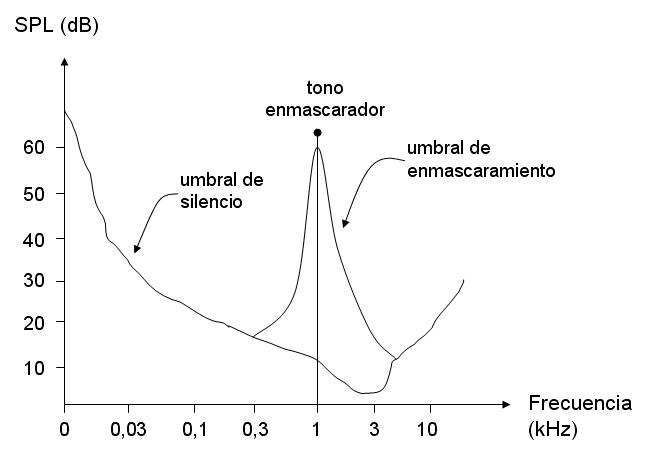
\includegraphics[width=0.9\textwidth]{figures/enmascaramiento.png}
    \caption{Umbral de enmascaramiento dado por un tono puro.}
\end{figure}


\textbf{Actividad práctica.} Usa Tone Generator para reproducir un tono de 1 kHz a 60 dB y otro de 1.1 kHz a 20 dB simultáneamente. Nota cómo el tono más fuerte (masker) dificulta escuchar el más débil (signal).

\section{Sonidos impulsivos e inteligibilidad}

\subsection{Sensibilidad temporal}
Sonidos breves ($<$50 ms), como consonantes (5–15 ms), requieren 10–15 dB más para percibirse con igual sonoridad que sonidos largos. En salas reverberantes, los ecos dificultan la percepción de estas consonantes.

\subsection{Índice de inteligibilidad}
La \textbf{inteligibilidad del habla} (IL\%) depende de la relación señal-ruido (SNR) y el tiempo de reverberación ($T_{60}$):
\[
\text{IL\%} \approx 100 \frac{\text{SNR} - \text{SNR}_{50}}{30}, \quad \text{SNR}_{50} \approx 2 \, \text{dB}.
\]
Por ejemplo, una SNR de 12 dB da $\approx$67\% de inteligibilidad.

\begin{quote}
    \textbf{Ejemplo clínico.} En un aula con reverberación alta ($T_{60}$ $>$ 1 s), los niños con hipoacusia tienen dificultad para entender palabras debido a la baja inteligibilidad.
\end{quote}

\section{Efecto de precedencia (Haas)}
El cerebro fusiona un sonido directo con sus reflexiones si llegan dentro de $<$50 ms, mejorando la sonoridad sin afectar la localización. Retardos de 15–20 ms son ideales en sistemas de refuerzo sonoro (como altavoces en auditorios).

\begin{quote}
    \textbf{Ejemplo clínico.} En una sala de conferencias, los altavoces deben retrasarse $<$20 ms respecto a la voz del orador para que los pacientes con audífonos perciban un sonido claro y localizado.
\end{quote}

\section{Localización binaural}

\subsection{Pistas físicas}
El cerebro usa dos pistas principales para localizar sonidos:
\begin{itemize}
    \item \textbf{Diferencia interaural de tiempo (DIT):} Retardo entre oídos (máximo $\approx$0.69 ms), efectivo para frecuencias $<$1.5 kHz.
    \item \textbf{Diferencia interaural de intensidad (DII):} Atenuación por la sombra de la cabeza (hasta 20 dB a 6 kHz).
\end{itemize}

\subsection{Pistas espectrales monaurales}
La forma del pabellón altera el espectro del sonido, ayudando a detectar la altura (arriba/abajo).

\begin{quote}
    \textbf{Ejemplo clínico.} Un audífono direccional usa DIT y DII para mejorar la localización en entornos ruidosos, ayudando al paciente a enfocarse en una conversación.
\end{quote}

\begin{figure}[h]
    \centering
    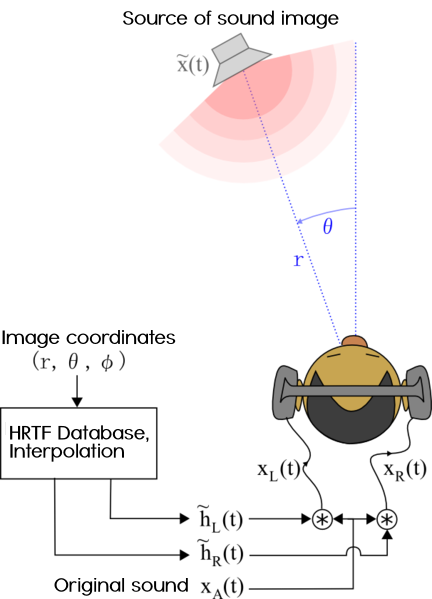
\includegraphics[width=0.5\textwidth]{figures/localizacion_fuentes.png}
    \caption{Sistema de localización binaural.}
    \label{localizacion_fuentes}
\end{figure}

\section{Efecto cocktail party}
El cerebro agrupa sonidos por similitud espectral y espacial, permitiendo enfocarse en una voz en un entorno ruidoso (como una fiesta). Los audífonos direccionales mejoran la SNR física ($\approx$6 dB), potenciando esta capacidad.

\begin{quote}
    \textbf{Ejemplo clínico.} Un paciente con audífonos direccionales puede seguir una conversación en un restaurante al reducir el ruido de fondo, aprovechando el efecto cocktail party.
\end{quote}

\textbf{Actividad práctica.} En un lugar ruidoso (como un café), intenta seguir una conversación cercana mientras escuchas ruido de fondo. Nota cómo tu cerebro “filtra” la voz objetivo, simulando el efecto cocktail party.

\section{Ejemplos prácticos}
\begin{enumerate}
    \item \textbf{Conversión a sones.} 60 fones = $2^{(60-40)/10} = 4$ sones.
    \item \textbf{Enmascaramiento.} Un masker de 60 dBSPL eleva el umbral de 20 dBSPL a $\approx$ 60 dBSPL, ya que la banda crítica integra la energía del masker.
    \item \textbf{DII.} Un tono de 6 kHz a 90° (sombra de cabeza) tiene una DII de $\approx$ 20 dB, haciendo que el sonido sea mucho más débil en el oído opuesto.
\end{enumerate}

\section{Ejercicios de autoevaluación}

\begin{enumerate}

    \item Explica por qué un ventilador que genera una señal de 31.5 Hz muestra una lectura menor en dBA que en dBZ. Usa la tabla de ponderaciones de la Unidad 5.
    \item Diseña un protocolo de enmascaramiento para una audiometría ósea a 1 kHz, considerando la banda crítica.
    \item Justifica por qué un sistema de refuerzo sonoro en una sala debe usar retardos $<$20 ms para mantener la localización.
    \item Usa Tone Generator para comparar un tono de 1 kHz a 60 dB con uno de 250 Hz a 60 dB. Explica la diferencia en sonoridad.
    
\end{enumerate}

\section{Recursos recomendados}

\begin{itemize}

    \item Video: \href{https://www.youtube.com/watch?v=csQkSZX9aJw&ab_channel=SrinathSrinivasan}{``Equal Loudness Contour explained''}. 
    \item App: Tone Generator (gratis). Prueba tonos y enmascaramiento.
    \item App: Audacity (gratis). Analiza espectros y timbres.
    \item Libro: B. C. J. Moore, \emph{An Introduction to the Psychology of Hearing}, capítulos 5–8.
    
\end{itemize}

\section*{Glosario}
\begin{description}
    \item[\textbf{Fon:}] Unidad de sonoridad, igual a dBSPL a 1 kHz.
    \item[\textbf{Son:}] Escala lineal de sonoridad (1 son = 40 fones).
    \item[\textbf{Banda crítica:}] Rango de frecuencias donde la energía se suma, afecta el enmascaramiento.
    \item[\textbf{DIT/DII:}] Diferencias interaurales de tiempo e intensidad, para localización.
    \item[\textbf{Efecto cocktail party:}] Capacidad de enfocar un sonido en un entorno ruidoso.
\end{description}

\section*{Resumen}
\begin{itemize}
    \item \textbf{Sonoridad:} Depende de la frecuencia y nivel (curvas isofónicas); se mide en fones y sones.
    \item \textbf{Atributos:} Altura (frecuencia), timbre (armónicos), duración (temporal).
    \item \textbf{Enmascaramiento:} Un sonido fuerte eleva el umbral de otro, clave en audiometrías.
    \item \textbf{Localización:} Usa DIT, DII y pistas monaurales; mejora con audífonos direccionales.
\end{itemize}

\bigskip
\noindent\emph{Conclusión.} La psicoacústica explica cómo percibimos el sonido más allá de su física, guiando el diseño de audífonos, pruebas audiométricas y entornos acústicos. Comprender la sonoridad, el enmascaramiento y la localización mejora la rehabilitación auditiva y la calidad de vida de los pacientes.



%%%%%%%%%%%%%%%%%%%%%%%%%%%%%%%%%%%%%%%%%%%%%%%%%%%%%%%%%%%%%%%%%%%%%%%%%%%%%%%%%%%%%%%%%%%%%%%%%%

% !TeX root = ../main.tex
\chapter{Unidad 8: Enfermedades auditivas, estudios diagnósticos y técnicas de rehabilitación}
\section*{Objetivo pedagógico}
\noindent\textbf{Objetivo.} Identificar las principales patologías auditivas (como tinnitus, presbiacusia y NIHL), comprender las pruebas diagnósticas (audiometría, OEA, PEA) y evaluar las opciones de rehabilitación tecnológica (audífonos, implantes cocleares) según el tipo y grado de pérdida auditiva, aplicando estos conocimientos en la práctica fonoaudiológica. Se incluyen ejemplos clínicos, actividades prácticas, recursos multimedia y ejercicios de autoevaluación.

\noindent\textbf{Pregunta inicial.} ¿Cómo se detecta una pérdida auditiva? ¿Qué opciones existen para ayudar a un paciente a escuchar mejor? ¡Esta unidad te ayudará a entender cómo diagnosticar y tratar problemas auditivos!

\section{Fatiga auditiva y daño inducido por ruido}

\subsection{Desplazamiento temporal del umbral (TTS)}
La exposición breve a ruidos fuertes ($>$85 dBSPL, como un concierto) eleva temporalmente el umbral de audición (TTS). La recuperación suele tomar 2–48 horas.

\begin{itemize}
    \item \textbf{Mecanismo:} Las células ciliadas externas (CCE) se agotan metabólicamente, causando edemas celulares.
    \item \textbf{Relevancia clínica:} TTS repetidos (por ejemplo, escuchar música alta frecuentemente) pueden llevar a daño permanente.
\end{itemize}

\begin{quote}
    \textbf{Ejemplo clínico.} Un adolescente que usa auriculares a 90 dB durante horas puede experimentar zumbidos temporales (TTS), un signo de alerta para prevenir daño permanente.
\end{quote}

\subsection{Pérdida auditiva inducida por ruido (NIHL)}
El \textbf{NIHL} (Noise-Induced Hearing Loss) es un daño permanente a las CCE, con un “notch” característico en 3–6 kHz en el audiograma. El riesgo depende del nivel equivalente ($L_{Aeq,8h}$) y los años de exposición.

\begin{quote}
    \textbf{Ejemplo clínico.} Un trabajador de fábrica expuesto a 90 dBA durante 20 años puede desarrollar un notch en 4 kHz, dificultando la comprensión de consonantes como ``s'' o ``f''.
\end{quote}

\paragraph{Normativa} La exposición laboral debe ser $<$85 dBA durante 8 horas (según OMS y normativas locales). Se usan protectores auditivos (NRR, Noise Reduction Rating) para reducir el riesgo.

\textbf{Actividad práctica.} Usa una app como Decibel X (gratis) para medir el nivel de ruido en un entorno ruidoso (como un café o concierto). Si supera 85 dBA, calcula cuánto tiempo es seguro permanecer sin protección.

\section{Trauma acústico y ototóxicos}
Un \textbf{trauma acústico} ($>$140 dBSPL, como una explosión) puede perforar el tímpano o dañar la membrana basilar. El tratamiento inmediato con corticosteroides puede minimizar la pérdida.

\begin{itemize}
    \item \textbf{Ototóxicos:} Fármacos como aminoglucósidos (gentamicina) o cisplatino dañan las CCE. Se monitorean con otoemisiones acústicas (OEA) y audiometría en altas frecuencias ($>$8 kHz).
\end{itemize}

\begin{quote}
    \textbf{Ejemplo clínico.} Un paciente en quimioterapia con cisplatino necesita pruebas regulares de OEA para detectar daño coclear temprano y ajustar el tratamiento.
\end{quote}

\section{Tinnitus y presbiacusia}

\subsection{Tinnitus}
El \textbf{tinnitus} es la percepción de zumbidos o sonidos sin fuente externa (prevalencia: 10–15\%). Se asocia con plasticidad cortical tras daño auditivo.

\begin{description}
    \item[\textbf{Enmascaramiento:}] Ruido de banda ancha a 5–10 dB sobre el tinnitus reduce su percepción.
    \item[\textbf{TRT (Tinnitus Retraining Therapy):}] Combina consejería y ruido modulador para habituar al paciente al tinnitus.
\end{description}

\begin{quote}
    \textbf{Ejemplo clínico.} Un paciente con tinnitus a 4 kHz puede usar un audífono con ruido de enmascaramiento para aliviar la molestia durante el día.
\end{quote}

\subsection{Presbiacusia}
La \textbf{presbiacusia} es la pérdida auditiva relacionada con la edad, con una pendiente de más de 2 dB por década en frecuencias mayores a 2 kHz. Afecta la inteligibilidad del habla, especialmente en agudos.

\begin{quote}
    \textbf{Ejemplo clínico.} Un adulto mayor con presbiacusia necesita audífonos que amplifiquen frecuencias altas (2–8 kHz) sin retroalimentación, mejorando la comprensión de palabras.
\end{quote}

\begin{figure}[h]
    \centering
    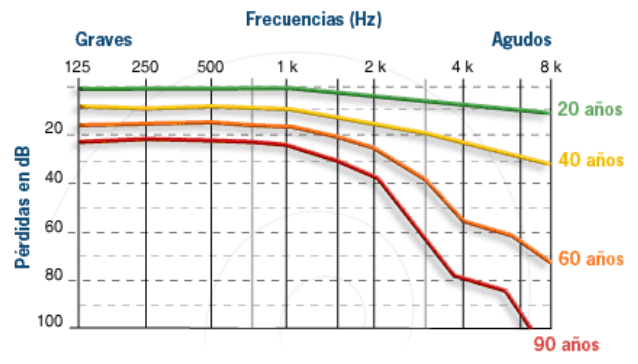
\includegraphics[width=0.9\textwidth]{figures/presbiacusia.png}
    \caption{Evolución de la presbiacusia con los años.}
    \label{fig:presbiacusia}
\end{figure}

\section{Estudios de la audición}

\subsection{Audiometría tonal}
Mide los umbrales de audición vía aérea y ósea (250 Hz–8 kHz). Clasificación de la pérdida:
\begin{itemize}
    \item Leve: 26–40 dB HL
    \item Moderada: 41–55 dB HL
    \item Moderada-severa: 56–70 dB HL
    \item Severa: 71–90 dB HL
    \item Profunda: $>$90 dB HL
\end{itemize}

\begin{quote}
    \textbf{Ejemplo clínico.} Un paciente con umbrales de 50 dB HL a 4 kHz (vía aérea) y 20 dB HL (vía ósea) tiene hipoacusia conductiva, posiblemente por otosclerosis.
\end{quote}

\subsection{Logoaudiometría}
Estudio que evalúa el reconocimiento de palabras (\%). La curva PI-PB (Phonetically Balanced) muestra el porcentaje de palabras entendidas según el nivel (dBSPL). Un “roll-over” (caída a niveles altos) indica lesión retrococlear.

\subsection{Timpanometría}
Mide la presión y compliancia del oído medio. Tipos:
\begin{itemize}
    \item \textbf{Tipo A:} Normal (pico de presión).
    \item \textbf{Tipo B:} Sin pico (otitis media serosa).
    \item \textbf{Tipo C:} Pico desplazado (disfunción de trompa de Eustaquio).
\end{itemize}

\begin{figure}[h]
    \centering
    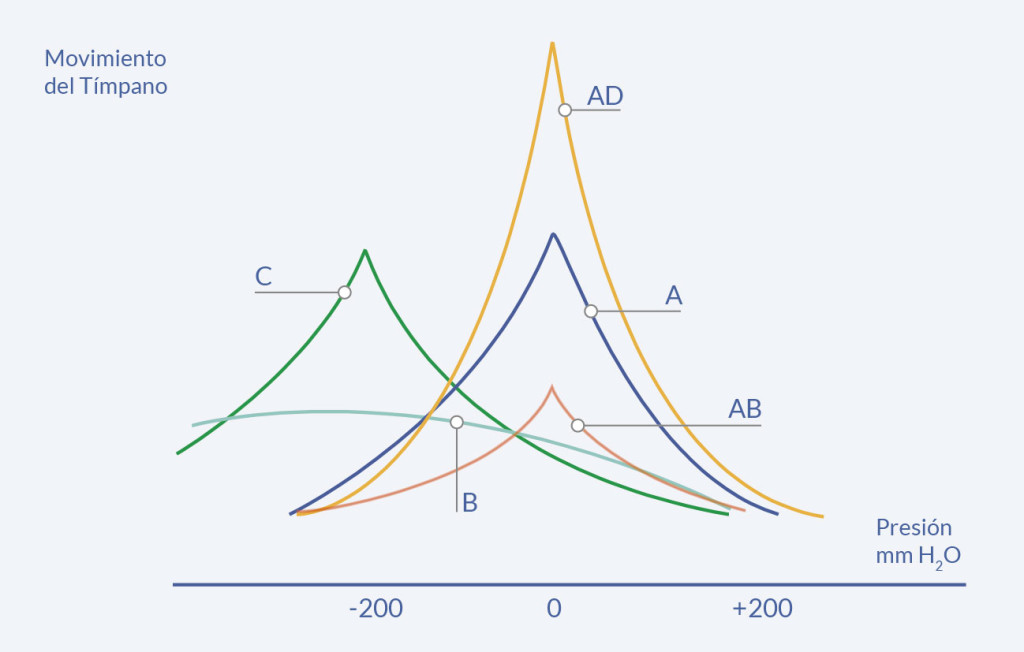
\includegraphics[width=0.9\textwidth]{figures/timpanometria.png}
    \caption{Tipos de resultados de timpanometrías.}
    \label{fig:timpanometria}
\end{figure}

\subsection{Acufenometría}
Compara el pitch y la intensidad del tinnitus con tonos puros para diseñar terapias de enmascaramiento.

\subsection{Pruebas electrofisiológicas}
\begin{itemize}
    \item \textbf{OEA (Otoemisiones Acústicas):} Evalúa las CCE. Usada en screening neonatal (dura $\approx$2 min).
    \item \textbf{PEA (Auditory Brainstem Response):} Mide latencias de ondas I–V ($<$10 ms) para evaluar la vía neural.
    \item \textbf{ECochG (Electrocochleografía):} Registra potenciales cocleares (SP, AP), útil en la enfermedad de Ménière.
\end{itemize}

\begin{table}[h]
    \centering
    \begin{tabular}{|l|c|c|c|}
        \hline
        \textbf{Prueba} & \textbf{Duración} & \textbf{Invasiva} & \textbf{Evalúa} \\
        \hline
        Audiometría & 10 min & No & Umbrales (conductiva/sensorial) \\
        OEA & 2 min & No & Función de CCE \\
        PEA & 15 min & No & Vía neural/retrococlear \\
        ECochG & 30 min & Sí* & Potenciales cocleares \\
        \hline
    \end{tabular}
    \caption{Comparación de estudios auditivos (*vía tímpano, requiere médico).}
\end{table}

\begin{quote}
    \textbf{Ejemplo clínico.} Un neonato con OEA ausente puede tener hipoacusia sensorioneural, confirmada con PEA para evaluar el nervio auditivo.
\end{quote}

\section{Rehabilitación tecnológica}

\subsection{Audífonos}
Amplifican sonidos con tecnología WDRC (Wide Dynamic Range Compression), hasta 70 dB de ganancia. Incluyen:
\begin{itemize}
    \item Micrófonos direccionales para mejorar la SNR.
    \item Cancelación de feedback (retroalimentación).
    \item Conectividad Bluetooth para teléfonos.
\end{itemize}

\begin{quote}
    \textbf{Ejemplo clínico.} Un paciente con presbiacusia usa un audífono que amplifica 2–8 kHz, con micrófonos direccionales para mejorar la inteligibilidad en entornos ruidosos.
\end{quote}

\subsection{Implante coclear (IC)}
Indicado para hipoacusia severa-profunda ($<$50\% reconocimiento de palabras). Usa 12–24 electrodos para estimular el nervio auditivo según el mapa tonotópico.

\subsection{Implantes osteointegrados (BAHA)}
Vibran la mastoides para hipoacusia conductiva (por ejemplo, atresia del CAE o infecciones crónicas).

\subsection{EAS (Electro-Acoustic Stimulation)}
Combina amplificación acústica ($<$1 kHz) con estimulación eléctrica ($>$1 kHz) para pacientes con audición residual en graves.


\section{Ejemplos prácticos}
\begin{enumerate}
    \item \textbf{Clasificación de pérdida.} Un paciente con un notch de 40 dB a 4 kHz y umbrales normales en 1 kHz tiene hipoacusia leve sensorioneural (NIHL). Consejería: usar protectores auditivos y monitorear anualmente.
    \item \textbf{Cálculo de $L_{Aeq,8h}$.} 95 dBA durante 1 h equivale a:
    \[
    L_{Aeq,8h} = 95 - 10 \log_{10}\left(\frac{8}{1}\right) \approx 86 \, \text{dBA}.
    \]
    \item \textbf{Ganancia necesaria.} Para un umbral de 60 dB a 2 kHz, la regla half-gain sugiere:
    \[
    \text{Ganancia} = \frac{60 - 20}{2} = 20 \, \text{dB}.
    \]
\end{enumerate}

\section{Ejercicios de autoevaluación}
\begin{enumerate}
    \item Compara el “notch” de NIHL con la pendiente de presbiacusia en un audiograma. ¿Cómo afecta cada uno a la inteligibilidad del habla?
    \item Describe los pasos de una prueba PEA y explica qué indica un retraso en la onda III.
    \item Enumera ventajas (mejor audición, conectividad) y limitaciones (costo, cirugía) del implante coclear en mayores de 70 años.
    \item Usa Decibel X para medir el ruido en un entorno (por ejemplo, un aula). Si supera 85 dBA, sugiere medidas preventivas.
\end{enumerate}

\section{Recursos recomendados}
\begin{itemize}
    \item Video: \href{https://www.youtube.com/watch?v=PnmRgyi4-dU&ab_channel=Cl%C3%ADnicaUniversidaddeNavarra}{``Implantes cocleares | Qué son, cómo funcionan y qué pacientes son candidatos''}.
    \item App: Tinnitus Relief (gratis). Ofrece sonidos para TRT.
    \item App: Decibel X (gratis). Mide niveles de ruido.
    \item Documento: OMS, \emph{Make Listening Safe} (PDF disponible en línea).
    \item Libro: J. Katz, \emph{Handbook of Clinical Audiology}, capítulos 10–12.
\end{itemize}

\section*{Glosario}
\begin{description}
    \item[\textbf{TTS:}] Desplazamiento temporal del umbral, reversible.
    \item[\textbf{NIHL:}] Pérdida auditiva inducida por ruido, con notch en 3–6 kHz.
    \item[\textbf{TRT:}] Terapia de reentrenamiento para tinnitus.
    \item[\textbf{PEA:}] Respuesta auditiva del tronco encefálico, mide latencias neurales.
    \item[\textbf{BAHA:}] Audífono anclado al hueso, para hipoacusia conductiva.
\end{description}

\section*{Resumen}
\begin{itemize}
    \item \textbf{Patologías:} NIHL (notch 3–6 kHz), presbiacusia (pendiente $>$2 kHz), tinnitus (zumbidos).
    \item \textbf{Diagnósticos:} Audiometría (umbrales), OEA (CCE), PEA (vía neural).
    \item \textbf{Rehabilitación:} Audífonos (WDRC), implantes cocleares (severa-profunda), BAHA/EAS.
\end{itemize}


\bigskip
\noindent\emph{Conclusión.} Comprender las patologías auditivas, las pruebas diagnósticas y las tecnologías de rehabilitación permite diseñar intervenciones personalizadas, mejorando la calidad de vida de los pacientes.



%%%%%%%%%%%%%%%%%%%%%%%%%%%%%%%%%%%%%%%%%%%%%%%%%%%%%%%%%%%%%%%%%%%%%%%%%%%%%%%%%%%%%%%%%%%%%%%%%%

% !TeX root = ../main.tex
\chapter{Unidad 9: Factores que afectan la propagación del sonido}

\section*{Objetivo pedagógico}
\noindent\textbf{Objetivo.} Comprender cómo la distancia, la direccionalidad de la fuente, las condiciones atmosféricas y las interacciones con superficies alteran la propagación del sonido, y aplicar estos conocimientos al diseño de espacios clínicos (como cabinas audiométricas) y al control de ruido ambiental en fonoaudiología. Se incluyen ejemplos clínicos, actividades prácticas, recursos multimedia y ejercicios de autoevaluación.

\noindent\textbf{Pregunta inicial.} ¿Por qué un sonido se escucha más débil a mayor distancia? ¿Cómo afecta el viento o una pared al sonido en una cabina audiométrica? ¡Esta unidad te ayudará a entender cómo viaja el sonido!

\section{Distancia a la fuente}

\subsection{Ley del cuadrado inverso}
En un campo libre (sin reflexiones), el nivel de presión sonora (SPL) disminuye 6 dB cada vez que se duplica la distancia desde la fuente:
\[
L_{p2} = L_{p1} - 20 \log_{10}\left(\frac{d_2}{d_1}\right).
\]
Esto se debe a que la energía se distribuye en una esfera más grande, como ondas en un estanque.

\begin{quote}
    \textbf{Ejemplo clínico.} En una audiometría de campo libre, un tono de 90 dBSPL a 0.5 m se reduce a 78 dBSPL a 1 m, lo que afecta la calibración del audiómetro según la distancia al paciente.
\end{quote}

\begin{figure}[h]
    \centering
    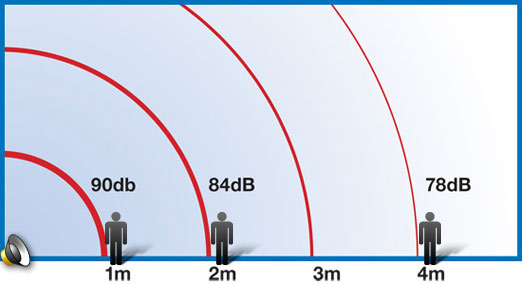
\includegraphics[width=0.9\textwidth]{figures/cuadrado_inverso.png}
    \caption{Representación de la ley del cuadrado inverso.}
    \label{fig:cuadrado-inverso}
\end{figure}


\section{Direccionalidad y factor \texorpdfstring{$Q$}{Q}}

\subsection{Definición}
El factor de directividad ($Q$) mide cómo una fuente concentra el sonido en una dirección:
\[
L_p = L_0 + 10 \log_{10} Q - 20 \log_{10}\left(\frac{d}{d_0}\right).
\]
Un $Q$ alto (como en una bocina) enfoca el sonido, aumentando el SPL en la dirección principal.

\begin{table}[h]
    \centering
    \begin{tabular}{|l|c|}
        \hline
        \textbf{Fuente} & \textbf{$Q$ aproximado} \\
        \hline
        Omnidireccional & 1 \\
        Hemiesférica (sobre suelo) & 2 \\
        Bocina direccional & 10–16 \\
        Line-array (banda media) & 30+ \\
        \hline
    \end{tabular}
    \caption{Valores típicos de directividad.}
\end{table}

\begin{quote}
    \textbf{Ejemplo clínico.} En una cabina audiométrica, se usan parlantes omnidireccionales ($Q=1$) para garantizar un campo sonoro uniforme, evitando variaciones por la posición del paciente.
\end{quote}

\begin{figure}[h]
    \centering
    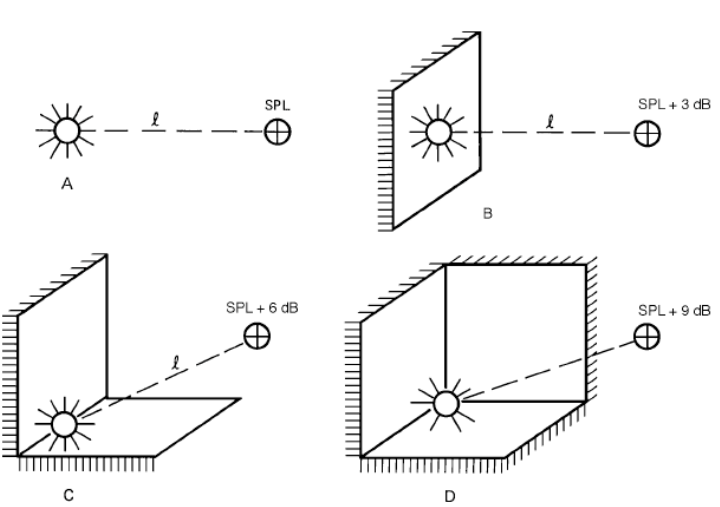
\includegraphics[width=0.9\textwidth]{figures/directividad.png}
    \caption{Diagrama de directividad de una fuente y cómo esta afecta a la propagación de la onda para $Q=1$, $Q=2$, $Q=3$ y $Q=4$}
    \label{directividad}
\end{figure}


\section{Condiciones atmosféricas}

\subsection{Temperatura}
La velocidad del sonido en el aire aumenta con la temperatura:
\[
c = 331 + 0.6T \, (\text{m/s}, \, T \text{ en °C}).
\]
Por ejemplo, a 30°C, $c \approx 349$ m/s. Los gradientes térmicos (como una inversión nocturna) curvan las ondas sonoras, aumentando el alcance al refractarlas hacia el suelo.

\begin{quote}
    \textbf{Ejemplo clínico.} En una evaluación de ruido ambiental cerca de una clínica, una inversión térmica nocturna puede hacer que el ruido de tráfico sea más audible, afectando las mediciones audiométricas.
\end{quote}

\subsection{Viento}
El viento modifica la velocidad efectiva del sonido:
\[
c' = c + u \cos \theta,
\]
donde $u$ es la velocidad del viento y $\theta$ el ángulo respecto al receptor. A favor del viento, el SPL aumenta; en contra, se reduce.

\subsection{Presión/altitud}
A mayor altitud, la menor densidad del aire reduce ligeramente el SPL (~1 dB por 1000 m).

\begin{quote}
    \textbf{Ejemplo clínico.} En una audiometría realizada a 2000 m de altitud, los niveles de salida de los auriculares pueden ser 2 dB más bajos, afectando la calibración del equipo y los resultados de la prueba.
\end{quote}

\section{Interacción con superficies}

\subsection{Reflexión y absorción}
Las superficies reflejan o absorben el sonido según su \textbf{coeficiente de absorción} ($\alpha$, de 0 a 1). La reverberación ($RT_{60}$, tiempo para que el sonido decaiga 60 dB) depende de la fórmula de Sabine:
\[
RT_{60} = \frac{0.161 V}{A}, \quad A = \sum (\alpha_i S_i),
\]
donde $V$ es el volumen del recinto y $A$ la absorción total.

\begin{quote}
    \textbf{Ejemplo clínico.} En una cabina audiométrica, se usan materiales absorbentes ($\alpha \approx 0.9$) para minimizar la reverberación, asegurando un campo libre.
\end{quote}

\subsection{Refracción}
El cambio de velocidad del sonido entre medios (por ejemplo, aire a vidrio) desvía las ondas, afectando el aislamiento en ventanas dobles.

\subsection{Difracción}
Las ondas rodean obstáculos si su tamaño es mucho menor que la longitud de onda ($\lambda$). Las frecuencias bajas (largas $\lambda$) difractan más, mientras que las altas quedan en sombra.

\begin{quote}
    \textbf{Ejemplo clínico.} En una clínica, una pared delgada no bloquea los graves (125 Hz, $\lambda \approx 2.7$ m), pero sí los agudos (4 kHz, $\lambda \approx 0.09$ m), afectando el aislamiento.
\end{quote}

\begin{figure}[h]
    \centering
    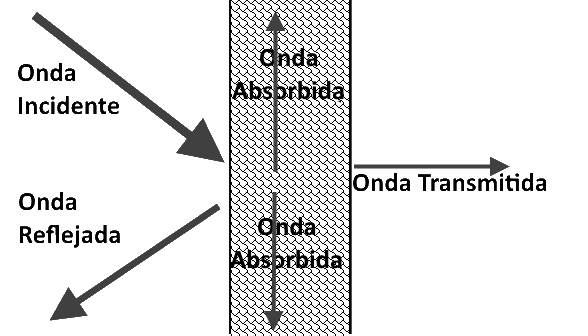
\includegraphics[width=0.9\textwidth]{figures/reflexion_absorcion.png}
    \caption{Fenómeno de reflexión y absorción de una onda sonora sobre una superficie.}
    \label{reflexion_absorcion}
\end{figure}

\section{Aislamiento e insonorización}
\begin{description}
    \item[\textbf{Aislamiento:}] Reduce la transmisión de sonido entre recintos, según la \textbf{ley de masas}:
    \[
    R \, (\text{dB}) = 20 \log_{10} (m f) - 47,
    \]
    donde $m$ es la masa superficial (kg/m²) y $f$ la frecuencia (Hz).
    \item[\textbf{Insonorización:}] Combina aislamiento y absorción para minimizar el ruido residual.
\end{description}

\begin{quote}
    \textbf{Ejemplo clínico.} Una cabina audiométrica requiere un aislamiento $>$70 dB a 1 kHz y un ruido residual $<$30 dBA para pruebas precisas.
\end{quote}

\section{Ejemplos prácticos}
\begin{enumerate}
    \item \textbf{SPL a distancia.} Un altavoz con $Q=4$ produce 90 dB a 2 m. A 8 m:
    \[
    L_p = 90 + 10 \log_{10} 4 - 20 \log_{10} \left(\frac{8}{2}\right) \approx 90 + 6 - 12 = 84 \, \text{dB}.
    \]
    \item \textbf{Velocidad y longitud de onda.} A 0°C, $c = 331$ m/s; a 30°C, $c = 349$ m/s. Para 500 Hz:
    \[
    \lambda_0 = \frac{331}{500} \approx 0.66 \, \text{m}, \quad \lambda_{30} = \frac{349}{500} \approx 0.70 \, \text{m}.
    \]
    \item \textbf{Altura de barrera.} Para atenuar 10 dB a 1 kHz ($\lambda \approx 0.34$ m), la barrera debe bloquear la línea de vista a 6 m. Usando la fórmula de difracción, altura mínima $\approx$1.5 m.
\end{enumerate}

\section{Ejercicios de autoevaluación}
\begin{enumerate}
    \item Explica por qué los sonidos graves (125 Hz) atraviesan paredes más fácilmente que los agudos (4 kHz).
    \item Describe cómo una inversión térmica nocturna aumenta el ruido de una fábrica en una clínica cercana.
    \item Calcula $RT_{60}$ para un aula de $8 \times 6 \times 3$ m ($V = 144$ m³) con $\bar{\alpha} = 0.25$. (\emph{Solución:} $RT_{60} \approx 0.72$ s.)
    \item Usa Decibel X para medir el ruido en una sala. Si supera 35 dBA, sugiere materiales absorbentes para reducir la reverberación.
\end{enumerate}

\section{Recursos recomendados}
\begin{itemize}
    \item Video: \href{https://www.youtube.com/watch?v=d8bODvda0NE&ab_channel=RyanHarne}{``Engineering Acoustics: 15. Outdoor Sound Propagation''}.
    \item App: Decibel X (gratis). Mide niveles de ruido.
    \item App: Tone Generator (gratis). Genera tonos para probar propagación.
    \item Libro: M. Raichel, \emph{Science and Applications of Acoustics}, capítulo 6.
    \item Norma: ISO 1996-2 (Medición de ruido ambiental).
\end{itemize}

\section*{Glosario}
\begin{description}
    \item[\textbf{$RT_{60}$:}] Tiempo para que el sonido decaiga 60 dB.
    \item[\textbf{$Q$:}] Factor de directividad, mide el enfoque del sonido.
    \item[\textbf{Sabine:}] Unidad de absorción (1 m² con $\alpha = 1$).
    \item[\textbf{Inversión térmica:}] Capa de aire caliente que refracta el sonido hacia el suelo.
\end{description}

\section*{Resumen}
\begin{itemize}
    \item \textbf{Distancia:} La ley del cuadrado inverso reduce el SPL 6 dB al duplicar la distancia.
    \item \textbf{Direccionalidad:} El factor $Q$ determina el enfoque del sonido.
    \item \textbf{Condiciones atmosféricas:} Temperatura, viento y altitud afectan la velocidad y el SPL.
    \item \textbf{Superficies:} Reflexión, absorción y difracción modifican el sonido.
    \item \textbf{Aislamiento:} La ley de masas y la insonorización son clave en cabinas audiométricas.
\end{itemize}


\bigskip
\noindent\emph{Conclusión.} Comprender cómo la distancia, la direccionalidad, las condiciones ambientales y las superficies afectan el sonido es esencial para diseñar cabinas audiométricas, optimizar la inteligibilidad del habla y controlar el ruido en entornos clínicos.



%%%%%%%%%%%%%%%%%%%%%%%%%%%%%%%%%%%%%%%%%%%%%%%%%%%%%%%%%%%%%%%%%%%%%%%%%%%%%%%%%%%%%%%%%%%%%%%%%%

% !TeX root = ../main.tex
\chapter{Unidad 10: El ruido y su caracterización}

\section*{Objetivo pedagógico}
\noindent\textbf{Objetivo.} Comprender los tipos de ruido, sus características espectrales y temporales, sus efectos en la salud auditiva y no auditiva, y las técnicas de medición, enmascaramiento y control, aplicándolos a la fonoaudiología (como en audiometrías y terapias para tinnitus) y al diseño de entornos clínicos. Se incluyen ejemplos clínicos, actividades prácticas, recursos multimedia y ejercicios de autoevaluación.

\noindent\textbf{Pregunta inicial.} ¿Por qué el ruido de una calle puede dificultar una conversación? ¿Cómo se mide y controla el ruido en una clínica? ¡Esta unidad te ayudará a entender el impacto del ruido y cómo manejarlo!

\section{Ruido versus sonido}
El \textbf{ruido} es un sonido no deseado o molesto, una percepción subjetiva. Por ejemplo, una canción puede ser música para un oyente y ruido para otro, dependiendo del contexto.

\begin{quote}
    \textbf{Ejemplo clínico.} En una cabina audiométrica, el ruido de un ventilador ($\approx$40 dBA) puede interferir con la detección de umbrales auditivos, mientras que para un paciente con tinnitus, un ruido controlado puede ser terapéutico.
\end{quote}

\section{Clasificación de los ruidos}
Los ruidos se clasifican según su duración, fuente y frecuencia:
\begin{description}
    \item[\textbf{Continuo:}] Nivel estable, como una turbina o una cascada.
    \item[\textbf{Intermitente:}] Varía con el tiempo, como el tráfico urbano.
    \item[\textbf{Impulsivo:}] Picos breves ($<$1 s), como un martillazo o disparo, medidos con $L_{\text{peak}}$.
    \item[\textbf{Ambiental:}] Mezcla de fuentes externas (tráfico, industria, ocio).
    \item[\textbf{Industrial:}] Máquinas en fábricas, con límite de 85 dBA por 8 h.
    \item[\textbf{Impacto:}] Impulsos repetidos, como en obras o canteras.
    \item[\textbf{Baja frecuencia:}] $<$200 Hz, atraviesa paredes y causa molestias fisiológicas (por ejemplo, vibraciones).
\end{description}

\begin{quote}
    \textbf{Ejemplo clínico.} Un paciente con hipoacusia expuesto a ruido impulsivo (como martillos neumáticos) puede desarrollar un desplazamiento temporal del umbral (TTS), detectable en audiometría.
\end{quote}

\section{Ruido aleatorio y su descripción estadística}
El ruido aleatorio es impredecible y se caracteriza por:
\begin{itemize}
    \item \textbf{RMS:} Valor efectivo de la señal.
    \item \textbf{$L_{eq}$:} Nivel equivalente, promedio ponderado en el tiempo.
    \item \textbf{Percentiles:} $L_{10}$ (nivel superado el 10\% del tiempo, picos); $L_{90}$ (nivel de fondo).
\end{itemize}

\subsection{Blanco, rosa y otros espectros}
\begin{itemize}
    \item \textbf{Ruido blanco:} Energía igual por Hz, suena “siseante” (como una radio mal sintonizada).
    \item \textbf{Ruido rosa:} Energía constante por octava (–3 dB/oct), suena más equilibrado, usado en calibraciones.
    \item \textbf{Ruido vocal:} Es un ruido blanco al que se le aplica un filtro pasa-bajos con frecuencia de corte en 1000 Hz, útil en logoaudiometría.
    \item \textbf{Ruido de banda estrecha (NBN):} Ancho $\approx$1/3 de octava, usado en enmascaramiento.
\end{itemize}

\begin{quote}
    \textbf{Ejemplo clínico.} En audiometría, se usa ruido vocal para evaluar la inteligibilidad del habla, mientras que el ruido de banda estrecha enmascara el oído contralateral.
\end{quote}

\begin{figure}[h]
    \centering
    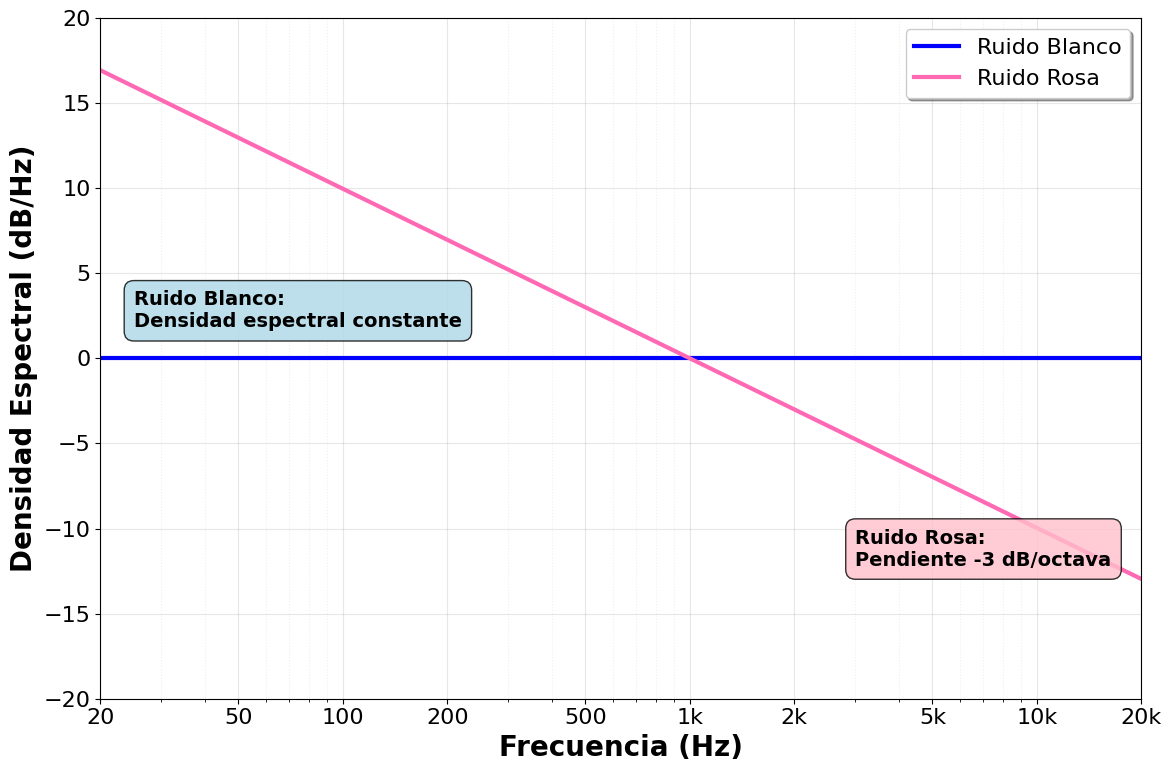
\includegraphics[width=1.0\textwidth]{figures/densidad_espectro_ruidos.png}
    \caption{Diferencias entre espectros de ruido blanco y rosa en escala logarítmica.}
    \label{densidad_espectro_ruidos}
\end{figure}


\textbf{Actividad práctica.} Usa Tone Generator (gratis) para escuchar ruido blanco y rosa. Nota cómo el ruido rosa suena más grave. Luego, graba un ruido ambiental con Audacity y observa su espectro.

\section{Técnica de enmascaramiento acústico}
El \textbf{enmascaramiento} usa ruido de banda estrecha (NBN) centrado en la frecuencia del tono a ocultar, elevando su umbral de detección. Es esencial en:
\begin{itemize}
    \item \textbf{Audiometría:} Enmascara el oído no evaluado para evitar respuestas cruzadas.
    \item \textbf{Terapia de tinnitus:} Ruido NBN a 5–10 dB sobre el tinnitus reduce su percepción.
\end{itemize}

\begin{quote}
    \textbf{Ejemplo clínico.} Para un paciente con tinnitus a 6 kHz, un audífono con NBN centrado en 6 kHz (ancho $\approx$1/3 octava) puede aliviar la molestia.
\end{quote}

\section{Efectos del ruido sobre la salud}
\begin{itemize}
    \item \textbf{Auditivos:} Pérdida auditiva inducida por ruido (NIHL, notch en 3–6 kHz), TTS, tinnitus.
    \item \textbf{No auditivos:} Estrés, insomnio, hipertensión (OMS, 2018: riesgo cardiovascular con $L_{den} > 65$ dB).
    \item \textbf{Cognitivos:} Disminución del rendimiento escolar en aulas con $L_{eq} > 65$ dB.
\end{itemize}

\begin{quote}
    \textbf{Ejemplo clínico.} Un niño en un aula ruidosa ($L_{eq} = 70$ dB) puede tener dificultades para concentrarse, afectando su aprendizaje del lenguaje.
\end{quote}

\section{Normativas y métricas}

\begin{table}[h]
    \centering
    \begin{tabular}{|l|c|c|}
        \hline
        \textbf{Entidad} & \textbf{Parámetro} & \textbf{Límite} \\
        \hline
        OMS (residencial, día) & $L_{\text{day}}$ & 55 dBA \\
        OMS (noche) & $L_{\text{night}}$ & 45 dBA \\
        ISO 1996-1/-2 & $L_{\text{den}}$ & 65 dBA \\
        OSHA (laboral) & $L_{Aeq,8h}$ & 85 dBA \\
        \hline
    \end{tabular}
    \caption{Valores guía de ruido ambiental y laboral.}
\end{table}

\subsection{Sonómetros y ponderación}
Los sonómetros clase 1 miden con ponderaciones A, C o Z y filtros temporales:
\begin{itemize}
    \item \textbf{Fast (125 ms):} Para ruidos continuos o intermitentes.
    \item \textbf{Slow (1 s):} Para promedios estables.
    \item \textbf{Impulse:} Para picos rápidos ($L_{\text{peak}}$).
\end{itemize}

\begin{quote}
    \textbf{Ejemplo clínico.} En una cabina audiométrica, un sonómetro con ponderación A verifica que el ruido de fondo sea $<$30 dBA, garantizando pruebas precisas.
\end{quote}

\section{Control y mitigación del ruido}
\begin{enumerate}
    \item \textbf{Fuente:} Silenciar máquinas, reducir velocidad, mantenimiento.
    \item \textbf{Trayecto:} Usar barreras acústicas, pantallas porosas, aislamiento (ley de masas).
    \item \textbf{Receptor:} Protectores auditivos (tapones, orejeras). Doble protección si $L_{\text{peak}} > 105$ dB.
\end{enumerate}

\begin{quote}
    \textbf{Ejemplo clínico.} En una clínica cerca de una calle ruidosa, se instalan ventanas dobles (aislamiento) y cortinas absorbentes para mantener el ruido $<$30 dBA en la cabina.
\end{quote}


\section{Ejemplos prácticos}
\begin{enumerate}
    \item \textbf{Cálculo de $L_{eq,1h}$.} Lecturas de 88, 92, 86, 90 dBA (impulsos, 15 min cada una):
    \[
    L_{eq,1h} = 10 \log_{10} \left( \frac{10^{88/10} + 10^{92/10} + 10^{86/10} + 10^{90/10}}{4} \right) \approx 89.5 \, \text{dBA}.
    \]
    \item \textbf{Atenuación de barrera.} Reducir la energía a 1/10 implica:
    \[
    \Delta L = 10 \log_{10} \left(\frac{1}{0.1}\right) = 10 \, \text{dB}.
    \]
    \item \textbf{Enmascaramiento de tinnitus.} Para 6 kHz, usar NBN centrado en 6 kHz (ancho $\approx$1/3 octava, 5–10 dB sobre el tinnitus), ajustado vía acufenometría.
\end{enumerate}

\section{Ejercicios de autoevaluación}
\begin{enumerate}
    \item Explica por qué el ruido rosa es preferido para calibrar sistemas de audio en comparación con el ruido blanco.
    \item Compara la molestia de un ruido continuo de 70 dBA con un ruido impulsivo de $L_{eq} = 55$ dBA y picos de 90 dB.
    \item Enumera tres materiales con $\alpha > 0.8$ a 1 kHz (por ejemplo, espuma acústica, cortinas gruesas, paneles perforados) y su uso en una clínica.
    \item Usa Decibel X para medir el ruido en un aula. Si $L_{eq} > 65$ dB, sugiere medidas de mitigación.
\end{enumerate}

\section{Recursos recomendados}
\begin{itemize}
    \item Video: \href{https://www.youtube.com/watch?v=Qkb2yRKJxSc&ab_channel=AudioUniversity}{``White Noise vs Pink Noise''}.
    \item App: Decibel X (gratis). Mide niveles de ruido y $L_{eq}$.
    \item App: Tone Generator (gratis). Genera ruidos blanco y rosa.
    \item Software: Room EQ Wizard (gratis). Analiza espectros y reverberación.
    \item Documento: OMS, \emph{Environmental Noise Guidelines} (2018, PDF en línea).
\end{itemize}

\section*{Glosario}
\begin{description}
    \item[\textbf{$L_{Aeq}$:}] Nivel equivalente de presión sonora ponderado A.
    \item[\textbf{$L_{\text{peak}}$:}] Nivel máximo instantáneo de un impulso.
    \item[\textbf{NBN:}] Ruido de banda estrecha, usado en enmascaramiento.
    \item[\textbf{Notch:}] Muesca en el audiograma, típica de NIHL.
\end{description}

\section*{Resumen}
\begin{itemize}
    \item \textbf{Tipos de ruido:} Continuo, intermitente, impulsivo, ambiental, baja frecuencia.
    \item \textbf{Caracterización:} Ruido blanco (plano), rosa (–3 dB/oct), vocal, NBN.
    \item \textbf{Efectos:} NIHL, tinnitus, estrés, problemas cognitivos.
    \item \textbf{Control:} Mitigación en fuente, trayecto y receptor; normativas OMS/OSHA.
\end{itemize}


\bigskip
\noindent\emph{Conclusión.} Caracterizar y controlar el ruido es clave para proteger la salud auditiva, mejorar la inteligibilidad del habla y diseñar entornos clínicos óptimos, como cabinas audiométricas. Estos conocimientos son esenciales en fonoaudiología para diagnósticos precisos y terapias efectivas, como el tratamiento del tinnitus.



%%%%%%%%%%%%%%%%%%%%%%%%%%%%%%%%%%%%%%%%%%%%%%%%%%%%%%%%%%%%%%%%%%%%%%%%%%%%%%%%%%%%%%%%%%%%%%%%%%


\end{document}
